\documentclass[12pt]{scrartcl}
\usepackage[scale=1.5]{ccicons}
\usepackage[notextcomp]{kpfonts} 
\usepackage[margin=0.5in]{geometry}
\usepackage{amsthm,amssymb,amsmath}
\usepackage{graphicx}
\usepackage{subcaption}
\usepackage{enumitem}
\usepackage{bm}
\usepackage{tabu}
\usepackage{mathtools}
\usepackage{tikz}
\usepackage{tikz-3dplot}
\usepackage{xcolor}
\usepackage{colortbl}
\usepackage{wasysym}



\usepackage{color}
\definecolor{darkblue}{rgb}{0, 0, .6}
\definecolor{grey}{rgb}{.7, .7, .7}
\usepackage[breaklinks]{hyperref}
\hypersetup{
	colorlinks=true,
	linkcolor=darkblue,
	anchorcolor=darkblue,
	citecolor=darkblue,
	pagecolor=darkblue,
	urlcolor=darkblue,
	pdftitle={},
	pdfauthor={}
}
\usepackage{fancyhdr}
%\thispagestyle{fancy}
%\lhead{}
%\chead{}
%\rhead{}
%\lfoot{}%\scriptsize This work is licensed under the \href{http://creativecommons.org/licenses/by-sa/3.0/us/}{Creative Commons Attribution-Share Alike 3.0 License}.} 
%\cfoot{}
%\rfoot{\ccbysa}
\renewcommand{\headrulewidth}{.4pt}
%\renewcommand{\footrulewidth}{.4pt}

\theoremstyle{definition}
\newtheorem{theorem}{Theorem}
\newtheorem*{theorem*}{Theorem}
\newtheorem{acknowledgement}[theorem]{Acknowledgement}
\newtheorem{algorithm}[theorem]{Algorithm}
\newtheorem{axiom}[theorem]{Axiom}
\newtheorem{case}[theorem]{Case}
\newtheorem{claim}[theorem]{Claim}
\newtheorem*{claim*}{Claim}
\newtheorem{conclusion}[theorem]{Conclusion}
\newtheorem{condition}[theorem]{Condition}
\newtheorem{conjecture}[theorem]{Conjecture}
\newtheorem{corollary}[theorem]{Corollary}
\newtheorem{criterion}[theorem]{Criterion}
\newtheorem{definition}[theorem]{Definition}
\newtheorem{example}[theorem]{Example}
\newtheorem{exercise}[theorem]{Exercise}
\newtheorem{journal}[theorem]{Journal}
\newtheorem{lemma}[theorem]{Lemma}
\newtheorem{notation}[theorem]{Notation}
\newtheorem{problem}[theorem]{Problem}
\newtheorem*{problem*}{Problem}
\newtheorem{proposition}[theorem]{Proposition}
\newtheorem{remark}[theorem]{Remark}
%\newtheorem{solution}[theorem]{Solution}
\newtheorem{summary}[theorem]{Summary}
\newtheorem{skeleton}[theorem]{Skeleton Proof}
\newtheorem{activity}[theorem]{Activity}
\newtheorem{intuitivedef}[theorem]{Intuitive Definition}

\DeclareMathOperator{\spn}{span}
\DeclareMathOperator{\Char}{Characteristic}
\DeclareMathOperator{\Aut}{Aut}
\DeclareMathOperator{\stab}{Stab}
\DeclareMathOperator{\Stab}{Stab}
\DeclareMathOperator{\orb}{\mathcal{O}}
\DeclareMathOperator{\lcm}{lcm}
\DeclareMathOperator{\gl}{GL}
\DeclareMathOperator{\Ker}{Ker}
\DeclareMathOperator{\Z}{\mathbb{Z}}
\DeclareMathOperator{\C}{\mathbb{C}}
\DeclareMathOperator{\R}{\mathbb{R}}
\DeclareMathOperator{\N}{\mathbb{N}}
\DeclareMathOperator{\Q}{\mathbb{Q}}
\DeclareMathOperator{\A}{\mathbb{A}}
\DeclareMathOperator{\Gal}{Gal}
\DeclareMathOperator{\PS}{\mathcal{P}}
\DeclareMathOperator{\acc}{acc}


\newenvironment{solution}{\begin{proof}[Solution]}{\end{proof}}
\newcommand{\comment}[1]{%
  \text{\phantom{(#1)}} \tag{#1}
}


%Useful for cut and paste
%\begin{enumerate}[label=\rm{(\alph*)}]

\begin{document}

%%%%%%%%%%%%%%%%% Day 1 %%%%%%%%%%%%%%%%%%%%
%\noindent
%	Introduce yourself to the other people at your table and ask each other the following questions record your answers on one of the whiteboards at your table:
%	\begin{enumerate}
%		\item What year are you? (i.e. Freshman, Sophomore, etc)
%		\item What is the first letter of your last name?
%		\item What is your favorite movie that you have seen in the past 12 months?
%		\item How many miles away is your home from Tucson (driving)?
%		\item How many hours do you spend on your phone per day? 
%	\end{enumerate}
%
%\newpage
%\noindent
%In your groups decide whether the following are categorical or numerical variables:
%\begin{enumerate}[leftmargin=!,labelindent=1.5cm,itemindent=-15pt]
%	\item The mode of transportation you take to class
%	\item The area code of your cell phone number
%	\item The number on the back of a UA basketball players jersey
%	\item The gas mileage of a car
%\end{enumerate}
%
%\newpage
%\noindent
%The following is the first initial of the last name of everyone in the class. Using this information create a frequency and relative frequency chart that represents this data with the following categories: A, B, C, D, E, F--Z.
%\begin{center}
%	\begin{tabular}{llllllllll}
%M & N & G & S & G & H & Q & T & G & R \\
%P & D & R & C & L & B & D & R & S & Z \\
%C & J & K & R & S & L & P & T & E & K \\
%M & C & M & P & P & D & M & C & M & T \\
%W & M & D & I & H & C & G & J & E & M \\
%R & Y & G &   &   &   &   &   &   &  
%\end{tabular}
%\end{center}

%%%%%%%%%%%%%%%%% Day 2 %%%%%%%%%%%%%%%%
%Recall last class we created a frequency and relative frequency table for the class standing of the students in our class. It looked something like this:\\
%	\begin{center}
%	\begin{tabular}{l|l|l}
%		
%		          & Frequency & Relative Frequency \\ \hline
%		Freshman  & 33        & 0.600              \\ \hline
%		Sophomore & 10        & 0.182              \\ \hline
%		Junior    & 4         & 0.073              \\ \hline
%		Senior    & 8         & 0.145              \\ \hline
%		Total     & 55        & 1                  \\ 
%	\end{tabular}	
%	\end{center}
%	Use this to answer the following questions on the white board at your table as a group.
%	
%	\begin{enumerate}
%		\item Draw a bar graph that represents the frequency column.
%		\item Draw a bar graph that represents the relative frequency column.
%		\item What differences are there between the two graphs you created?
%		\item How many students are freshman OR sophomores?
%		\item What proportion of students are freshman AND seniors?
%	\end{enumerate}
%	
%\newpage
%\noindent
%As a group create a table on your whiteboard that displays the information that was just posted in the announcement in D2L.
%
%\newpage
%\noindent
%Let's study this one now.\\
%	
%	\begin{center}
%		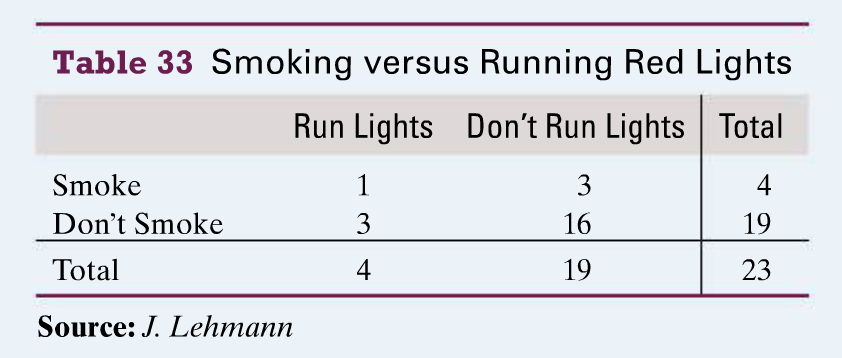
\includegraphics{twoway}
%	\end{center}
%	
%
%\noindent
%	Answer the following questions about the data presented above:
%	\begin{enumerate}
%		\item How many people don't smoke?
%		\item How many people run red lights?
%		\item What proportion of people smoke AND don't run red lights?
%		\item What proportion of people don't smoke OR run lights?	
%	\end{enumerate}
%
%\newpage
%\noindent
%The two different types of variables are:\\
%	\hspace{2cm} \underline{\hspace{2cm}} which describes data that is \underline{\hspace{2cm}}\\
%	\underline{\hspace{2cm}} which describes data that is \underline{\hspace{2cm}}.\\
%	
%	\noindent
%	We use the following things to describe categorical data:
%	\begin{itemize}
%		\item \underline{\hspace{5cm}}
%		\item \underline{\hspace{5cm}}
%		\item \underline{\hspace{5cm}}
%		\item \underline{\hspace{5cm}}
%		\item \underline{\hspace{5cm}}
%		\item \underline{\hspace{5cm}}
%	\end{itemize}

%%%%%%%%%%%%%%%%%%%%% Day 3 %%%%%%%%%%%%%%%%%%%%
%\noindent
%The following is a table that compares class standing to types of body art from a undergraduate students at a certain university. 
%
%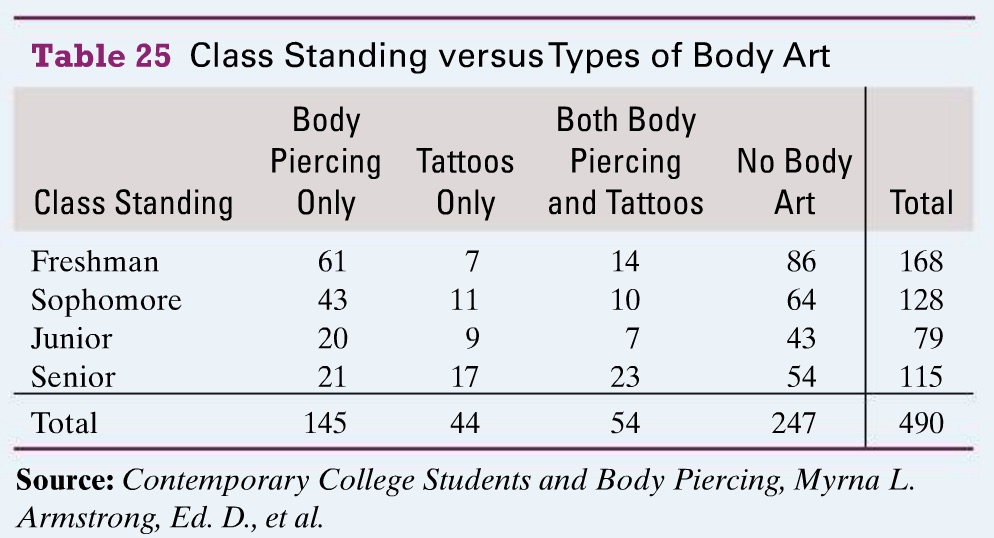
\includegraphics[scale=0.45]{bodyartclassstanding}
%
%\noindent
%Use it to answer these questions:
%\begin{enumerate}
%	\item How many students have Body Piercings Only AND are Sophomores?
%	\item What proportion of students have no body art AND Seniors?
%	\item How many students are Sophomores OR Tattoos Only?
%	\item What proportion of students have Both Body Piercing and Tattoos OR are Juniors?
%\end{enumerate}
%
%\newpage
%\noindent
%Consider the following numerical variables and decide what types of numbers are used to measure them (whole numbers, fractions, etc)
%\begin{enumerate}
%	\item Age
%	\item Number of times a person went out last year
%	\item Gas Mileage of a car
%	\item Height
%	\item Number of strings on a musical instrument
%	\item Clothing sizes
%\end{enumerate}
%
%\newpage
%\noindent
%The following is a dotplot that represents the asking price for certain four bedroom houses in thousands of dollars in Arkon, Ohio:
%\begin{center}
%	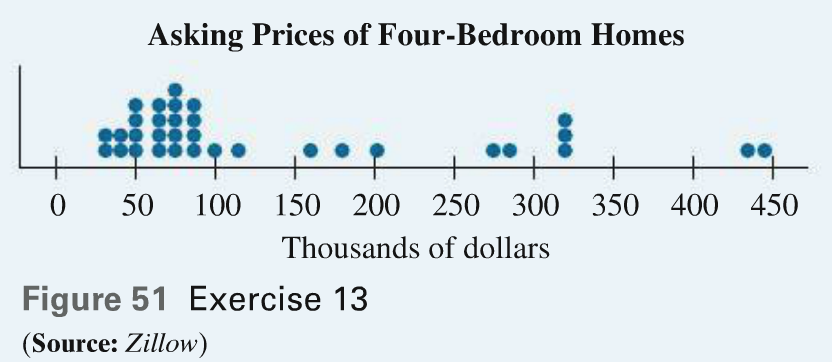
\includegraphics{dotplot}
%\end{center}
%
%\noindent
%Answer the following questions about this data:
%\begin{enumerate}
%	\item What is the frequency of the number of four bedroom houses that sold for \$75,000?
%	\item Are any dates much larger or smaller than the others? Why do you think this might be?
%	\item What house price is larger than or equal to 20\% of all other states? $\ldots$ 50\% of all other states? $\ldots$ 80\% of all other states?
%\end{enumerate}
%
%\newpage
%\noindent
%Using the same data as the previous example work with your group to answer the following questions:
%\begin{center}
%	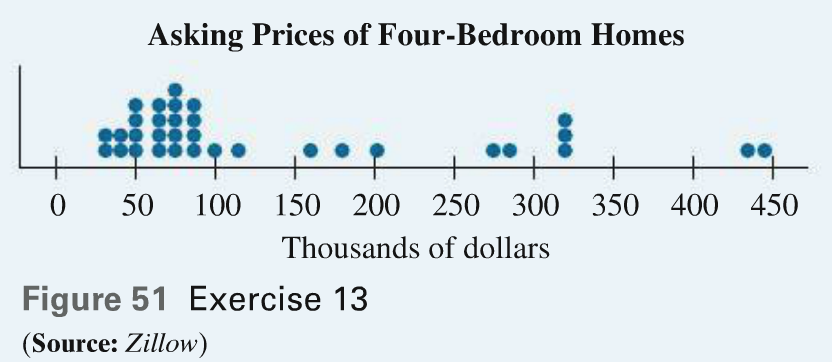
\includegraphics{dotplot}
%\end{center}
%\begin{enumerate}
%	\item Make a stemplot (sometimes known as a stem and leaf) plot that represents this data.
%	\item What value represents the 25th percentile? $\ldots$ the 60th percentile? $\ldots$ the 90th percentile?
%\end{enumerate}
%
%\newpage
%\section*{Announcements}
%\subsection*{Thursday, January 18}
%\begin{itemize}
%	\item MyMathLab Section 3.1 due 11:30pm
%\end{itemize}
%
%\subsection*{Sunday, January 21}
%\begin{itemize}
%	\item MyMathLab Section 3.2 due 11:30pm
%\end{itemize}
%
%\subsection*{Tuesday, January 23}
%\begin{itemize}
%	\item MyMathLab Section 3.3 due 11:30pm
%\end{itemize}

%%%%%%%%%%%%%%%%%%%% Day 4 %%%%%%%%%%%%%%%%%%%%
%Using the data as the last example from class work with your group to answer the following questions:
%	
%	\begin{center}
%	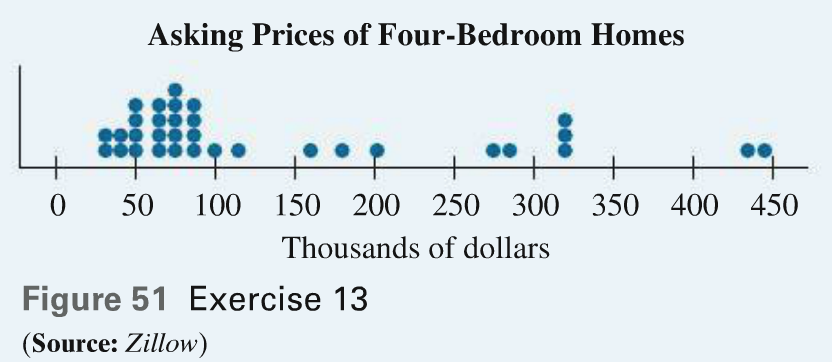
\includegraphics[]{dotplot}
%	\end{center}
%
%\begin{enumerate}
%	\item Make a stemplot (sometimes known as a stem and leaf) plot that represents this data.
%	\item What value represents the 25th percentile? $\ldots$ the 60th percentile? $\ldots$ the 90th percentile?
%\end{enumerate}
%
%\newpage
%\noindent
%Using the data from the data from the intro activity create a frequency table that has a lower class limit of 25 and a class width of 50. Here we are working with thousands of dollars.
%\begin{center}
%	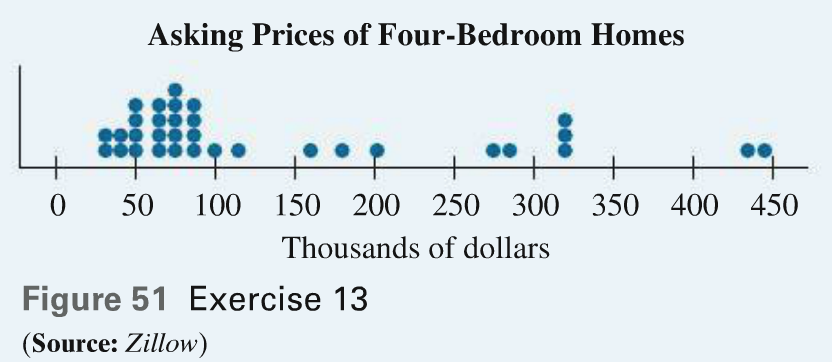
\includegraphics{dotplot}
%\end{center}
%
%\newpage
%\begin{figure}[h!]
%\centering
%  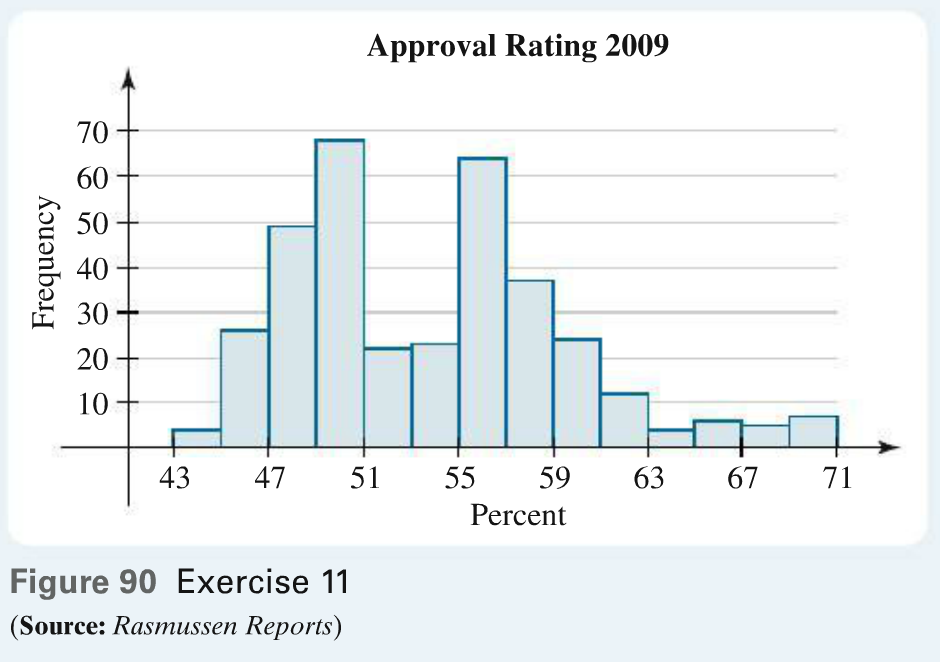
\includegraphics[]{Bimodal}
%\end{figure}%	
%\begin{figure}[h!]
%  \centering
%  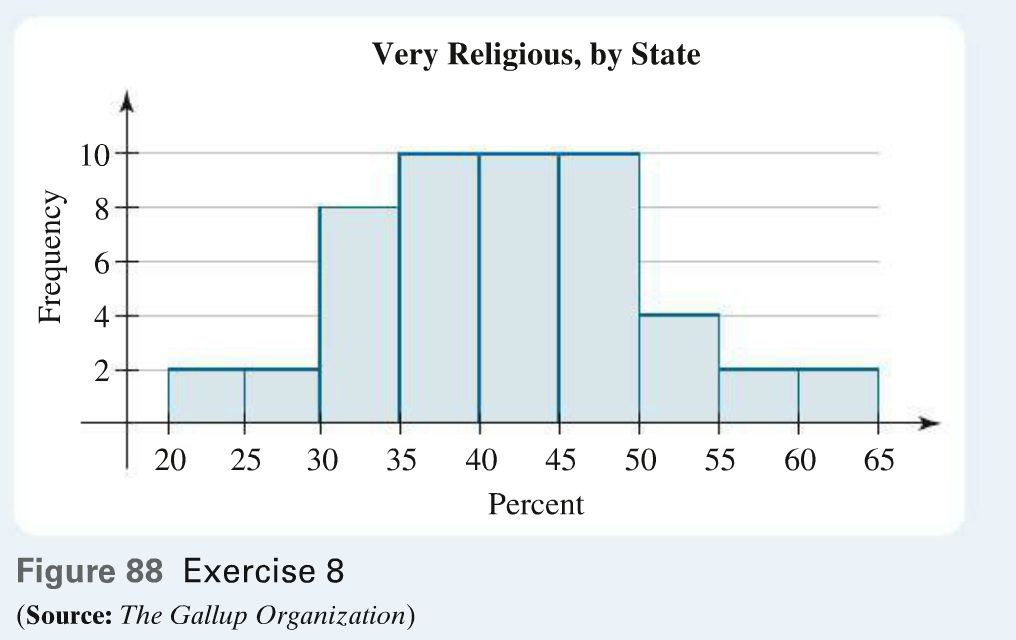
\includegraphics[]{Symmetric}
%\end{figure}
%
%\newpage
%\noindent
%
%\begin{figure}[h!]
%  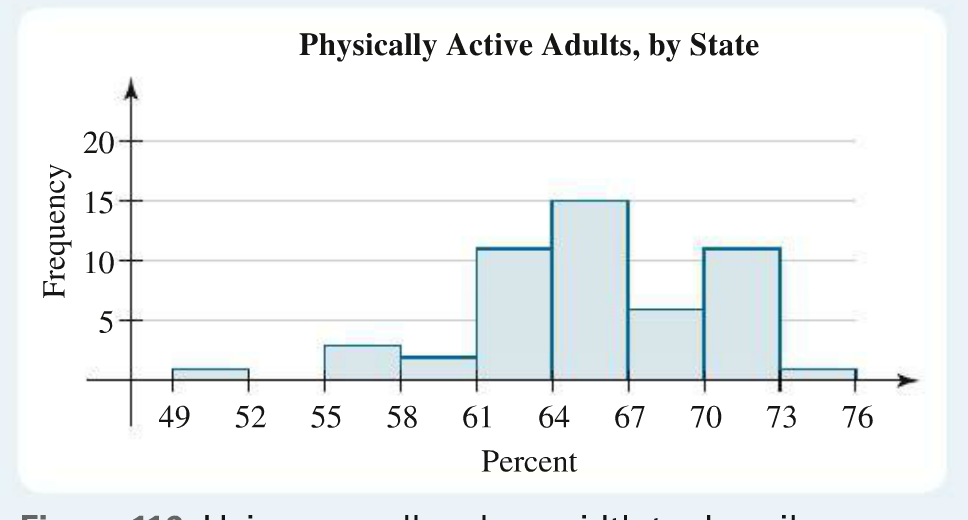
\includegraphics[]{Left_Skewed}
%\end{figure}%	
%\begin{figure}[h!]
%  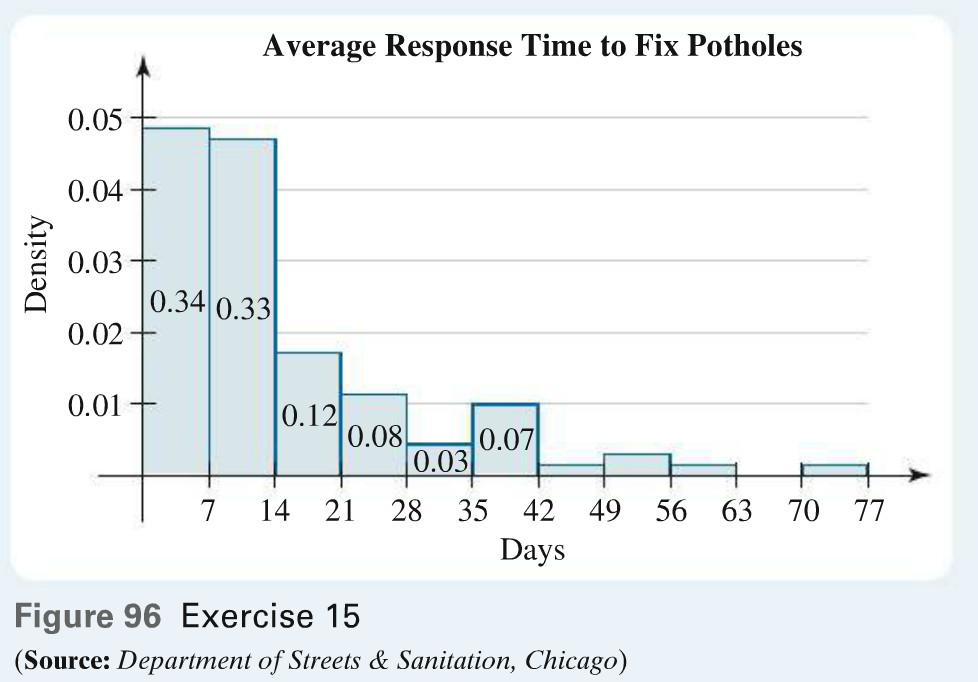
\includegraphics[]{Right_Skewed}
%\end{figure}
%	
%\newpage
%\noindent
%Scientists visited 30 sites along the Colorado River and counted the number of seedlings of Cottonwood trees. The following is their counts:
%\begin{center}
%	\begin{tabular}{llllll}
%48  & 49  & 52  & 54  & 54  & 57  \\
%61  & 63  & 67  & 67  & 69  & 70  \\
%70  & 72  & 73  & 73  & 76  & 79  \\
%79  & 83  & 85  & 87  & 96  & 98  \\
%103 & 105 & 108 & 112 & 138 & 139
%\end{tabular}
%\end{center}
%
%\noindent
%\textbf{Even Numbered Tables:} Construct a histogram using classes that start at 48 and have a class width of 19.\\
%
%\noindent
%\textbf{Odd Numbered Tables:} Construct a histogram using classes that start at 48 and have a class width of 10.
%
%\newpage
%\noindent
%\begin{enumerate}
%	\item Are you here on time? \vspace{2.5cm}
%	\item What value represents the 50th percentile? \vspace{2.5cm}
%	\item If you are creating a histogram with a class/count table that starts at 12 and has a class width of 27, what is the upper bound of the first class? \vspace{2.5cm}
%	\item Looking at the following histogram describe its shape (unimodal, bimodal, multimodal, left skewed, right skewed, symmetric). \begin{center} 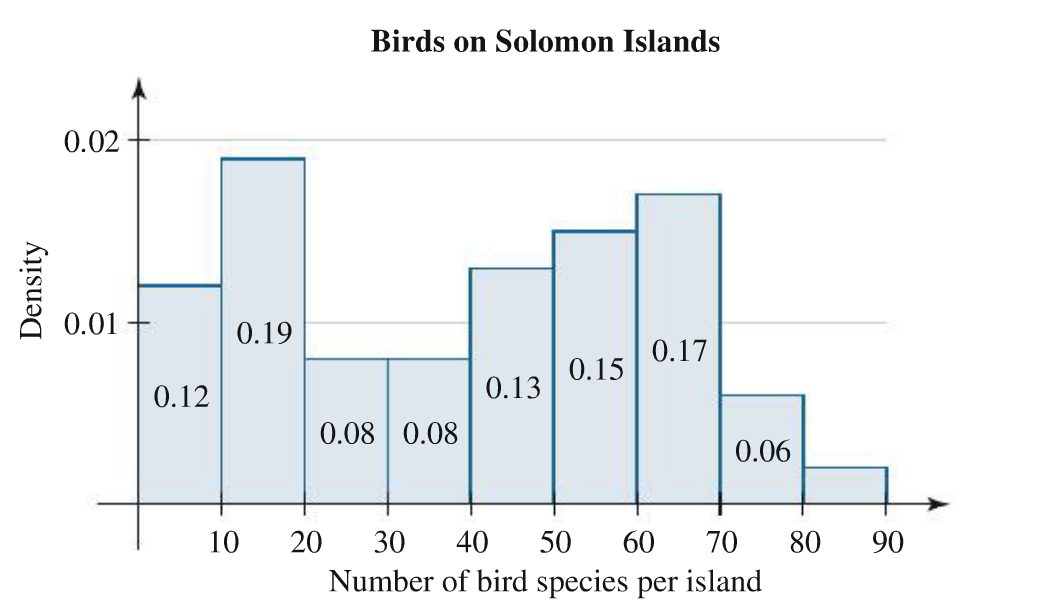
\includegraphics[scale=0.9]{histogramclicker} \end{center}
%\end{enumerate}
%
%\newpage
%\section*{Announcements}
%\subsection*{Tuesday, January 23}
%\begin{itemize}
%	\item MyMathLab Section 3.3 due 11:30pm
%\end{itemize}
%
%\subsection*{Thursday, January 25}
%\begin{itemize}
%	\item Quiz 1 in class (bring your laptop)
%\end{itemize}
%
%\subsection*{Sunday, January 28}
%\begin{itemize}
%	\item MyMathLab Section 3.4a due 11:30pm
%\end{itemize}

%%%%%%%%%%%%%%%%%%%% Day 5 %%%%%%%%%%%%%%%%%%%%

%\subsection*{Warm-Up/Intro Activity}
%\textbf{Copy the following into your notes and fill in the blanks.}\\
%
%\noindent
%A \underline{\hspace{5cm}} consists of names  or labels of groups of individuals.\bigskip\\
%
%\noindent
%A \underline{\hspace{5cm}} consists of measurable quantities that describe individuals.\bigskip\\
%
%\noindent
%We use a \underline{\hspace{5cm}} or a \underline{\hspace{5cm}} to display categorical variables in a readable format where the \underline{\hspace{5cm}} is the number of observations in that category and the \textbf{relative frequency} is calculated by \underline{\hspace{5cm}} and they sum to \underline{\hspace{5cm}}.\bigskip\\
%
%\noindent
%The following is a list of displays for categorical data:
%\begin{itemize}
%	\item 
%	\item
%	\item
%	\item
%	\item
%\end{itemize}
%
%\noindent
%When we use the word \textbf{AND} we are including observations that satisfy \underline{\hspace{5cm}} (2 words). Using the word \textbf{OR} we are including observations that satisfy \underline{\hspace{5cm}} (3 words).\bigskip \\
%
%\noindent
%A \textbf{discrete variable} is a \underline{\hspace{5cm}} variable that has \underline{\hspace{5cm}} between successive, possible values.\bigskip\\
%
%\noindent
%A \textbf{continuous variable} is a \underline{\hspace{5cm}} variable that can take on \underline{\hspace{5cm}} between two possible values.\bigskip\\
%
%\noindent
%The following is a list of displays for numerical data:
%\begin{itemize}
%	\item 
%	\item
%	\item
%	\item
%\end{itemize}
%\bigskip
%
%\noindent
%The \underline{\hspace{5cm}} of some data is a value (not necessarily a data value) that is bigger than or equal to k\% of the observations.\bigskip \\
%
%\noindent
%Draw a picture of a histogram that is:
%\begin{itemize}
%	\item unimodal
%	\item bimodal
%	\item multimodal
%	\item right skewed
%	\item left skewed
%\end{itemize}
%
%\newpage
%\noindent
%The following data are the numbers of endangered species in randomly selected African questions.\\
%\begin{center}
%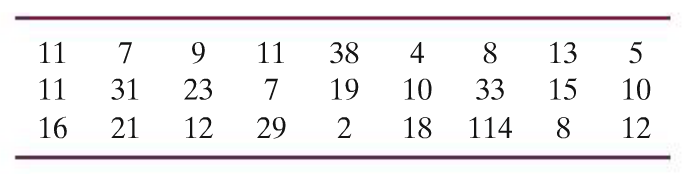
\includegraphics{africadata}
%\end{center}
%Use this data to answer the following questions:
%\begin{enumerate}
%	\item Construct a histogram that has a class width of 19 and starts at 2.
%	\item Describe the shape of the histogram.
%	\item Are there any outliers?
%	\item What class does the 50th percentile fall into? In relation to the histogram, where is the 50th percentile located?
%\end{enumerate}
%
%\newpage
%\begin{center}
%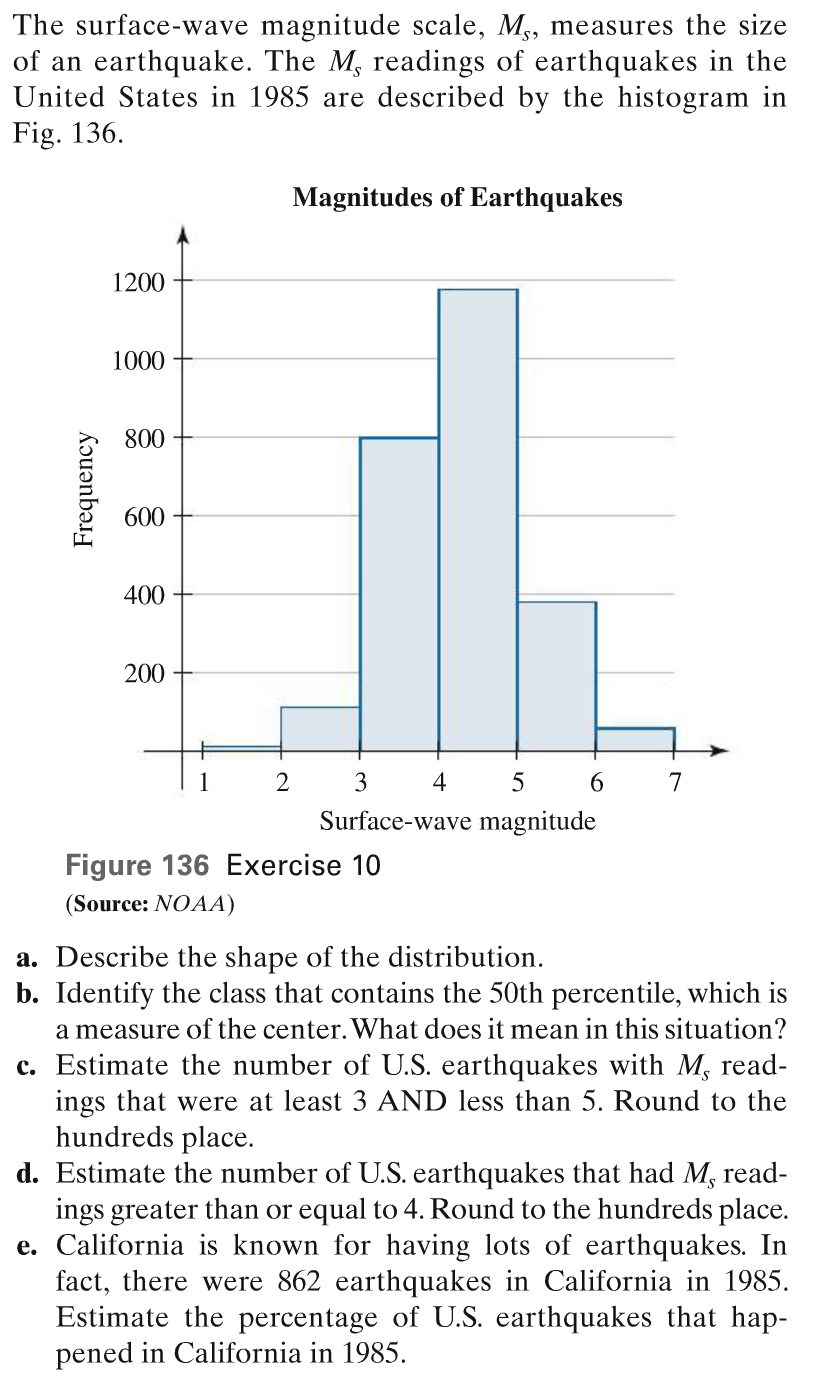
\includegraphics[scale=1.1]{Histogrampractice}	
%\end{center}
%
%\newpage
%\section*{Announcements}
%\subsection*{Sunday, January 28}
%\begin{itemize}
%	\item MyMathLab Section 3.4a due 11:30pm
%\end{itemize}
%
%\subsection*{Tuesday, January 30}
%\begin{itemize}
%	\item MyMathLab Section 3.4b due 11:30pm
%\end{itemize}
%
%\subsection*{Thursday, February 1}
%\begin{itemize}
%	\item Excel Project 1 due 11:30pm 
%\end{itemize}

%%%%%%%%%%%%%%%%%%%% Day 6 %%%%%%%%%%%%%%%%%%%%

%\noindent
%The following is the amount of money that Jos\'{e} spent on lunch the past 12 days at school.
%\begin{center}
%	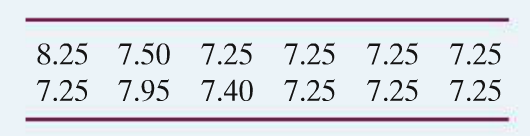
\includegraphics{LunchPrices}
%\end{center}
%Use this information to answer the following questions:
%\begin{enumerate}
%	\item Calculate the following in regards to the data:
%		\begin{itemize}
%			\item Mean
%			\item Median
%			\item Mode
%		\end{itemize}
%	\item Considering the above numbers, write a sentence that Jos\'{e} could use to persuade his parents that he isn't spending too much on lunch.
%	\item Now consider the perspective of Jos\'{e}'s parents, write a sentence that they could use to persuade Jos\'{e} he is spending too much on lunch.
%	\item Suppose instead on day 11 Jos\'{e} spent \$12.25 and on day 12 he spent \$10.50. Repeat the above exercises.
%\end{enumerate}
%
%\newpage
%\noindent
%Use this data to answer the following questions:
%\begin{center}
%	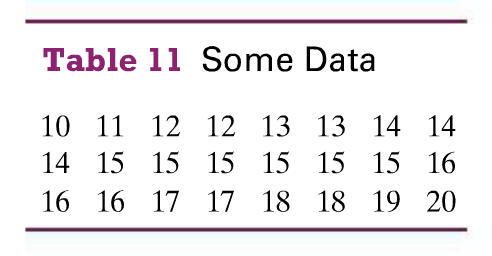
\includegraphics{MeanMedian}	
%\end{center}
%
%\begin{itemize}
%	\item For this activity you need your graphing calculator out.
%	\item Agree on one persons computer to use for this activity and open the MyMathLab textbook to page A-2 to find directions how to input data into a list.
%	\item Once the data is input into the list go to page A-4 to find directions on how to compute Mean, Median and other standard deviations of the data.
%\end{itemize}
%
%\begin{enumerate}
%	\item Record the Mean ($\overline{x}$) and Median (Med) on one of the white boards at your table. Create a histogram that represents this data with a class width of 2 that has a lower class limit of 10. (Remember if a data value falls on the border of a class we include it in the class it is the upper limit for)
%	\item Complete the following activity:
%		\begin{itemize}
%			\item \textbf{EVEN Tables:} Remove the top 3 values from the original data and replace them with the values 40, 40, 41
%			\item \textbf{ODD Tables:} Remove the bottom 3 values from the original data and replace them with the values 2, 2, 4.
%		\end{itemize}
%\end{enumerate}
%
%\newpage
%\noindent
%\begin{figure}[h!]
%\centering
%\begin{subfigure}{.5\textwidth}
%  \centering
%  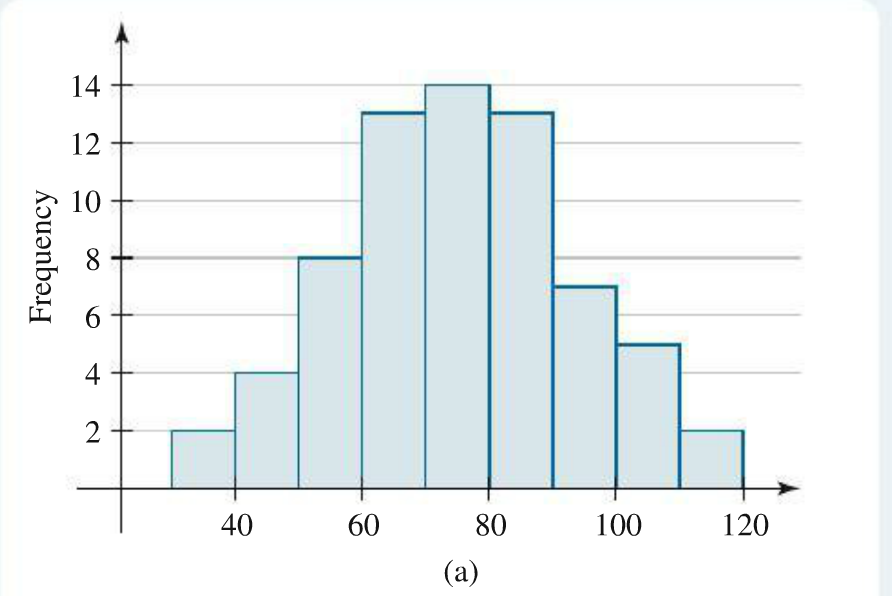
\includegraphics[scale=0.45]{Symmetric4}
%\end{subfigure}%	
%\begin{subfigure}{.5\textwidth}
%  \centering
%  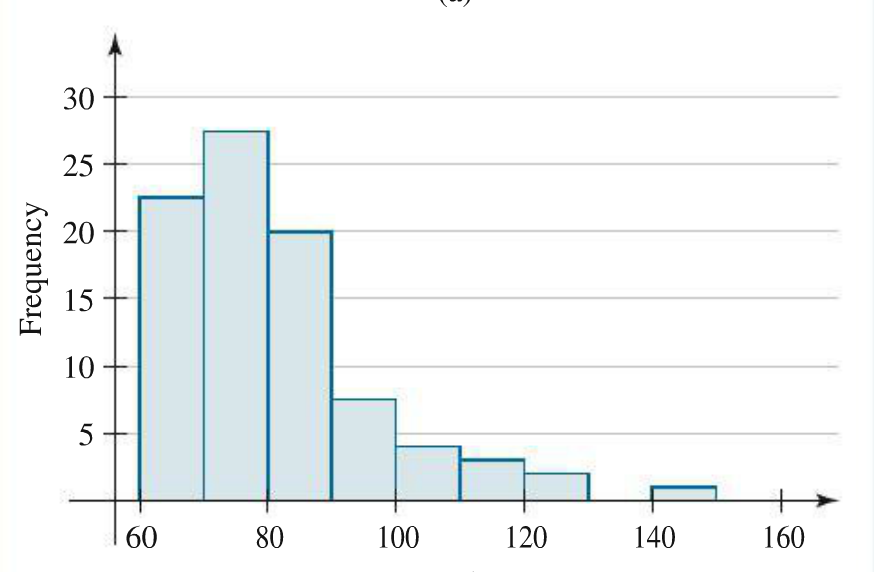
\includegraphics[scale=0.45]{RightSkewed4}
%\end{subfigure}
%\end{figure}
%
%\begin{center}
%	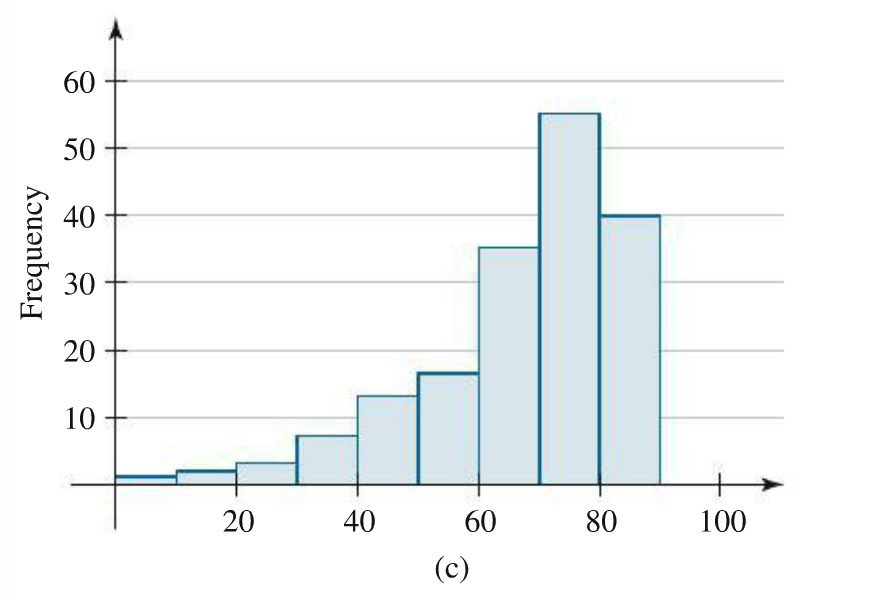
\includegraphics[scale=0.45]{LeftSkewed4}
%\end{center}
%
%\noindent
%Use the figures above to compare the mean and median for each set of data:\\
%
%\noindent
%Based on class discussion for each figure state whether the mean is equal to the median, the mean is less than the median or the mean is lower than the median.
%
%\newpage
%\noindent
%Are you here on time?
%
%\vspace{2.5cm}
%
%\noindent
%Calculate the mean of the following data: 2, 5, 8, 10
%
%\vspace{2.5cm}
%
%\noindent
%Calculate the median of the following data: 2, 5, 8, 10
%
%\vspace{2.5cm}
%
%\noindent
%For Figure (a): How is the mean related to the median?\\
%
%\noindent
%(A) Less Than \hspace{1cm} (B) Equal to \hspace{1cm} (C) Greater than
%
%
%\vspace{2.5cm}
%
%\noindent
%For Figure (b): How is the mean related to the median?\\
%
%\noindent
%(A) Less Than \hspace{1cm} (B) Equal to \hspace{1cm} (C) Greater than
%
%\vspace{2.5cm}
%
%\noindent
%For Figure (c): How is the mean related to the median?\\
%
%\noindent
%(A) Less Than \hspace{1cm} (B) Equal to \hspace{1cm} (C) Greater than
%	
%\end{document}

%%%%%%%%%%%%%%%%%%%% Day 7 %%%%%%%%%%%%%%%%%%%%

%\noindent
%Consider the following 3 data sets:
%\[ A=\{7,9,10,11,13\} \hspace{1cm} B=\{10,10,10,10,10\}\] \[ C=\{1,1,10,19,19\} \]
%
%\noindent
%Calculate the mean and median for these three sets and record them on your whiteboard.\\
%
%\newpage
%\noindent
%The following data is the number of calories in one slice ($\frac{1}{8}$th of a 14" Pizza) at Pizza Hut:
%
%\begin{center}
%	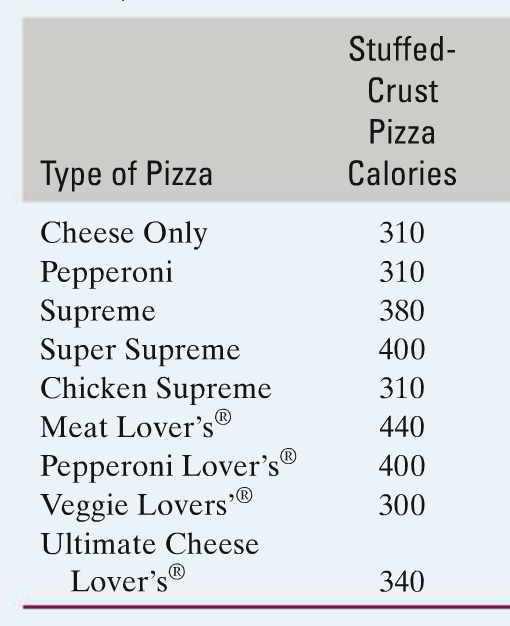
\includegraphics[scale=1]{StdDev}
%\end{center}
%
%\noindent
%Calculate the mean and standard deviation of the number of calories in one slice of pizza from Pizza Hut. Explain in context of the problem what this means.
%
%\newpage
%\noindent
%Recall one of the data sets from the beginning of class:
%\[A=\{7,9,10,11,13\} \]
%
%\noindent
%We found the following measurements regarding it:
%\begin{itemize}
%	\item $\overline{x}=10$
%	\item $M=10$
%	\item $R=6$
%	\item $s=2.236$
%\end{itemize}
%
%\noindent
%Answer the following questions:
%\begin{enumerate}
%	\item Add 5 to each of the data values in the set and calculate the mean, median, standard deviation and range for the new set of values. Write a sentence that explains how the new values compare to the original values.
%	\item Multiply each value by 5 and calculate the mean, median, standard deviation, and range for the new set of values. Write a sentence that explains how the new values compare to the original values.
%	\item Using what you found in the Problem 1 and 2 to write a sentence that generalizes your findings.
%\end{enumerate}
%
%\newpage
%
%Consider the following data set:
%
%\begin{center}
%	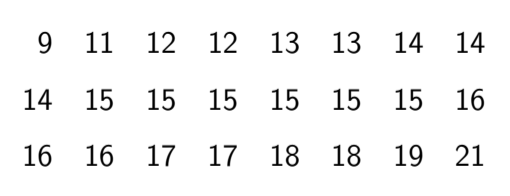
\includegraphics{EmpiricalRule}
%\end{center}
%
%Use it to answer the following questions:
%\begin{enumerate}
%	\item Calculate the mean and standard deviation for the given data.
%	\item Compute $\overline{x}-s$ and $\overline{x}+s$. Write a sentence that explains the computation you just completed.
%	\item How many observations lie within the values you computed above? What percentage of the overall observations is this?
%	\item Find the percentage of observations that lie within the values of $\overline{x}-2s$ and $\overline{x}+2s$.
%	\item Find the percentage of observations that lie with the values of $\overline{x}-3s$ and $\overline{x}+3s$.
%\end{enumerate}
%
%\newpage
%\noindent
%Consider the following histograms:
%\begin{center}
%  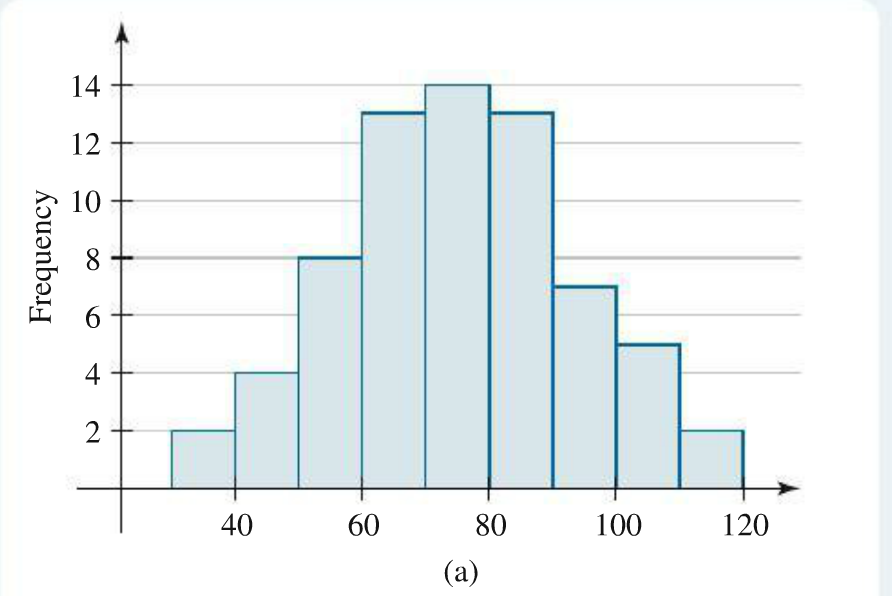
\includegraphics[scale=0.6]{Symmetric4}
%\end{center}
%
%\vspace{0.5cm}
%
%\begin{center}
%  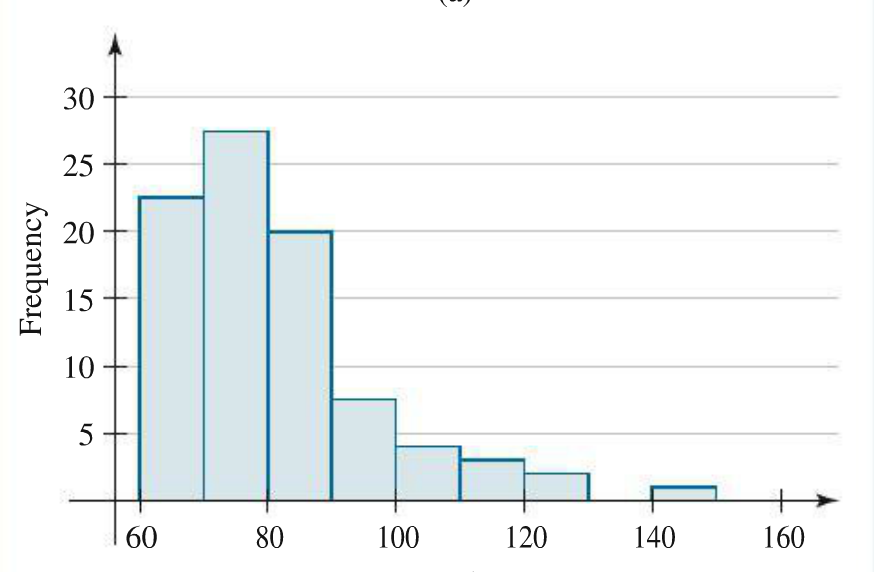
\includegraphics[scale=0.6]{RightSkewed4}
%\end{center}
%
%\vspace{0.5cm}
%
%\begin{center}
%	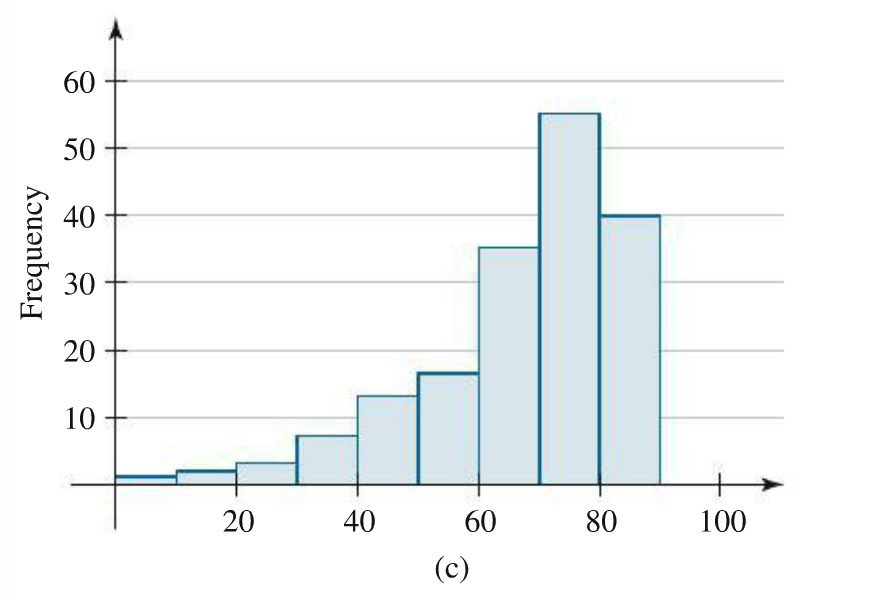
\includegraphics[scale=0.6]{LeftSkewed4}
%\end{center}
%
%
%\newpage
%\begin{center}
%  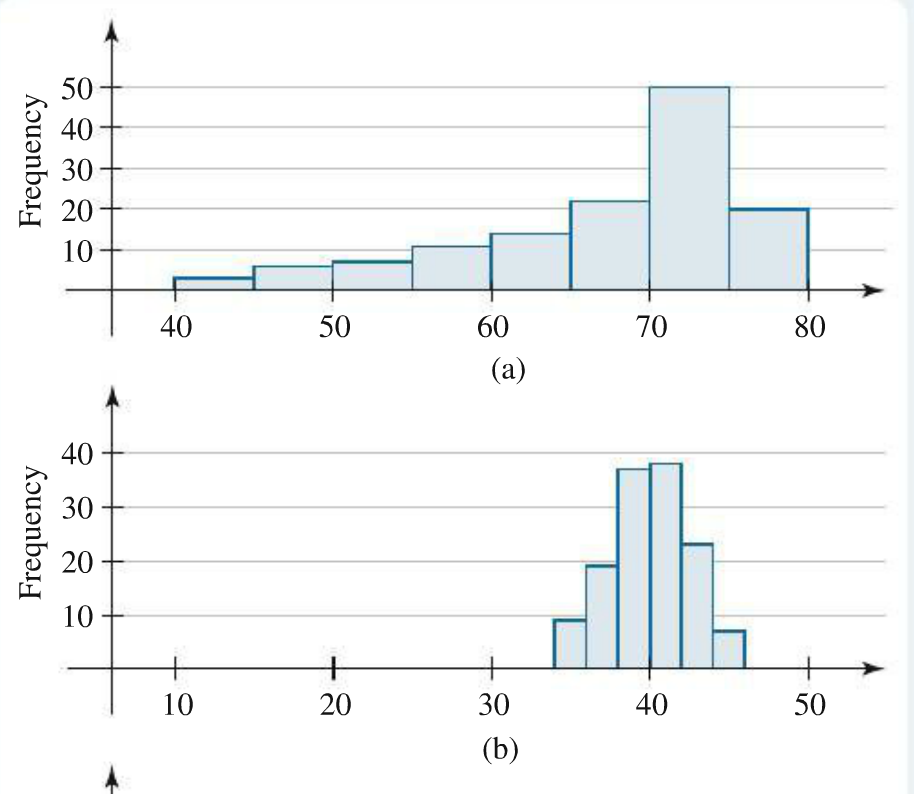
\includegraphics[scale=0.9]{MeasureofCSHistograms}
%\end{center}%	
%\begin{center}
%  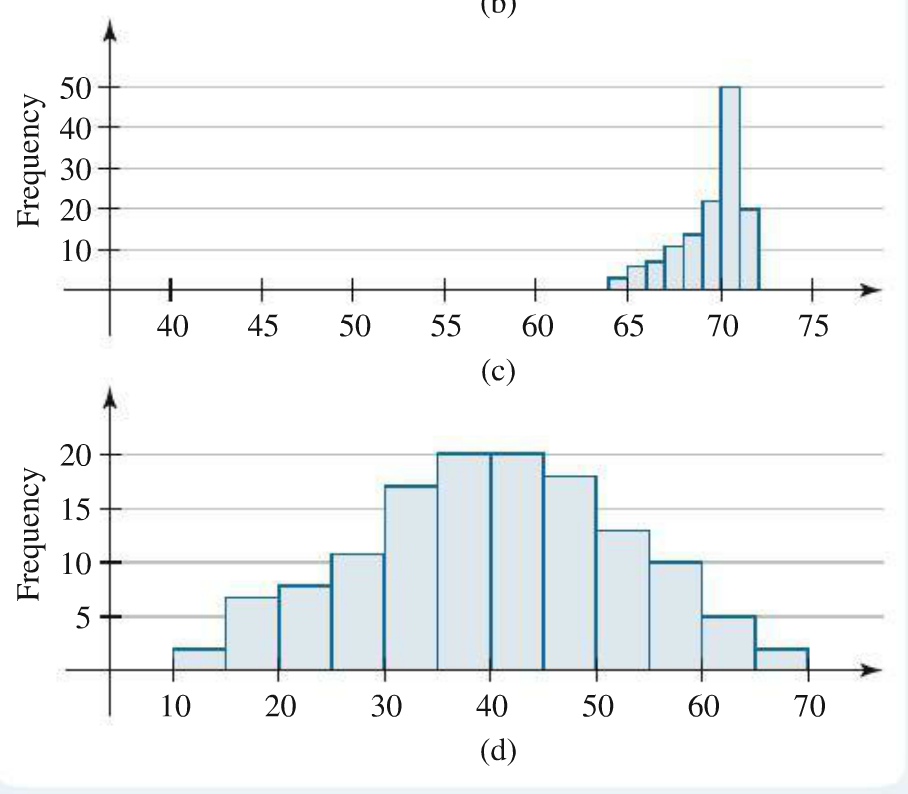
\includegraphics[scale=0.9]{MeasureofCSHistograms2}
%\end{center}


%%%%%%%%%%%%%%%%%%%% Day 8 %%%%%%%%%%%%%%%%%%%%

%\noindent
%Recall one of the data sets from last Thursday's class:
%\[A=\{7,9,10,11,13\} \]
%
%\noindent
%We found the following measurements regarding it:
%\begin{itemize}
%	\item $\overline{x}=10$
%	\item $m=10$
%	\item $R=6$
%	\item $s=2.236$
%\end{itemize}
%
%\noindent
%Answer the following questions:
%\begin{enumerate}
%	\item Add 5 to each of the data values in the set and calculate the mean, median, standard deviation and range for the new set of values. Write a sentence that explains how the new values compare to the original values.
%	\item multiply each value by 5 and calculate the mean, median, standard deviation, and range for the new set of values. Write a sentence that explains how the new values compare to the original values.
%	\item Using what you found in the Problem 1 and 2 to write a sentence that generalizes your findings.
%\end{enumerate}
%
%\newpage
%\noindent
%\begin{figure}[h!]
%\centering
%\begin{subfigure}{.5\textwidth}
%  \centering
%  \includegraphics[scale=0.45]{measureofCSHistograms}
%\end{subfigure}%	
%\begin{subfigure}{.5\textwidth}
%  \centering
%  \includegraphics[scale=0.45]{measureofCSHistograms2}
%\end{subfigure}
%\end{figure}
%
%\begin{enumerate}
%	\item $\overline{x}= 40$, $s=2.5$
%	\item $\overline{x}= 40$, $s=12.4$
%	\item $m=70$, $R=7.6$
%	\item $m=70$, $R=38$
%\end{enumerate}
%
%
%\newpage
%\noindent
%The following data is the 2013 monthly fuel consumption in millions of gallons by United Airlines.
%
%\begin{center}
%	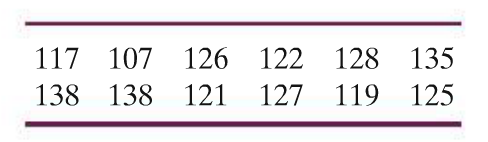
\includegraphics{BoxplotData}
%\end{center}
%
%\noindent
%Use this data to answer the following questions:
%\begin{enumerate}
%	\item Find the \textbf{minimum}, and \textbf{maximum} of the data
%	\item Find the \textbf{25th}, \textbf{50th} and \textbf{75th} percentiles
%	\item What is another name for the 50th percentile?
%	\item Using your graphing calculator calculate the mean, and standard deviation of this data
%	\item Scroll down in your one variable statistics and record the values seen for $Q_1$, $M$, and $Q_3$.
%	\item Compare these values to the values you found in Problem 2.
%	\item Based on your answer to Problems 2, 5 and 6. What conclusions can you make?
%\end{enumerate}
%
%\newpage
%\noindent
%Now that we have created a box plot answer the following questions:
%\begin{enumerate}
%	\item How many values are less than $Q_1$?
%	\item How many values are between $Q_1$ and $M$?
%	\item How many values are between $M$ and $Q_3$?
%	\item How many values are greater than $Q_3$?
%	\item Based on the answers you got above and your knowledge of percentiles what sort of generalization can we make about the number of data values that fall less than $Q_1$? between $Q_1$ and $M$? between $M$ and $Q_3$? greater than $Q_3$?
%\end{enumerate}
%
%\newpage
%\noindent
%Use the data from the beginning of the class to answer the following questions:
%
%\begin{center}
%	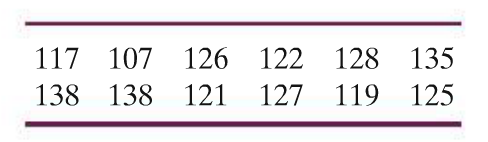
\includegraphics{BoxplotData}
%\end{center}
%
%\begin{enumerate}
%	\item Create a histogram with a class width of 5 that starts a 105.
%	\item Describe the shape of the histogram.
%	\item Compare the histogram to the box plot. 
%	\item Make a statement about how you can tell the shape of a distribution from a box plot.
%\end{enumerate}
%
%\newpage
%\noindent
%Use these two data sets to answer the following questions:
%
%\[ \text{Data Set 1:} 1, 3, 5, 7, 9, 11, 13, 15, 17\]
%\[ \text{Data Set 2:} 1, 3, 5, 7, 9, 16, 18, 20, 22\]
%
%\begin{enumerate}
%	\item Compare the two data sets: How are they similar? How are they different?
%	\item Draw boxplots for each of these sets of data.
%	\item Compare the min, $Q_1$, M, $Q_3$ and max. How are they similar? How are they different?
%\end{enumerate}
%
%\newpage
%\noindent
%Match the following histograms to the respective box plots. 
%
%\begin{center}
%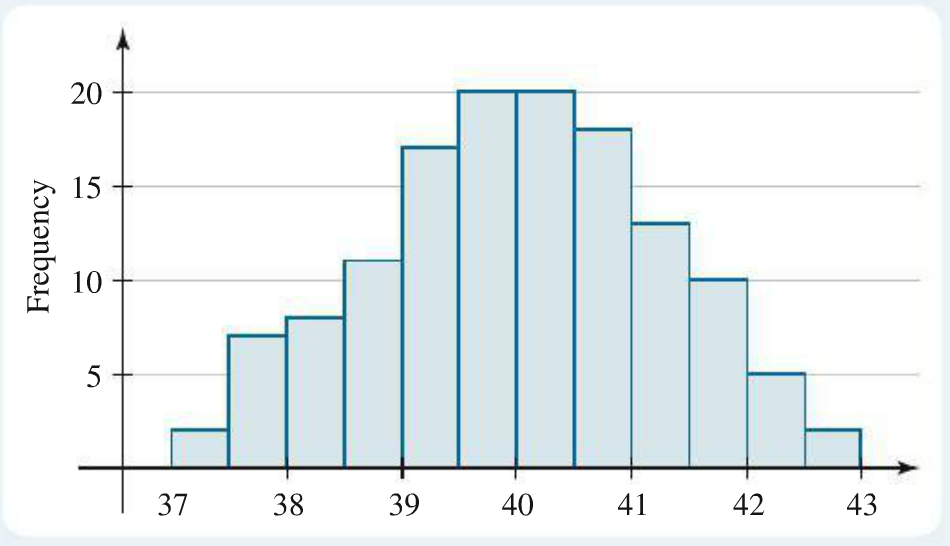
\includegraphics[scale=0.75]{Figure97}
%\end{center} \vspace{1cm}
%
%\begin{center}
%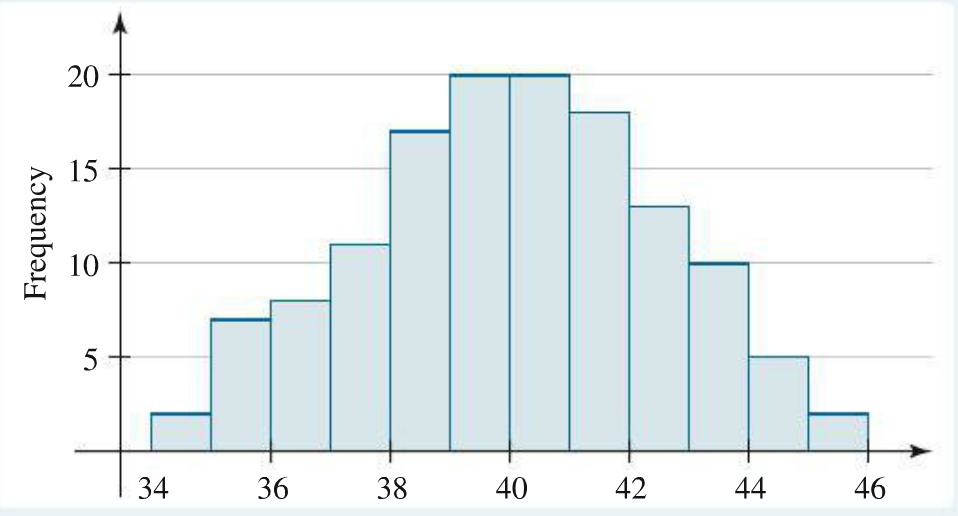
\includegraphics[scale=0.75]{Figure98}
%\end{center}\vspace{1cm}
%
%\begin{center}
%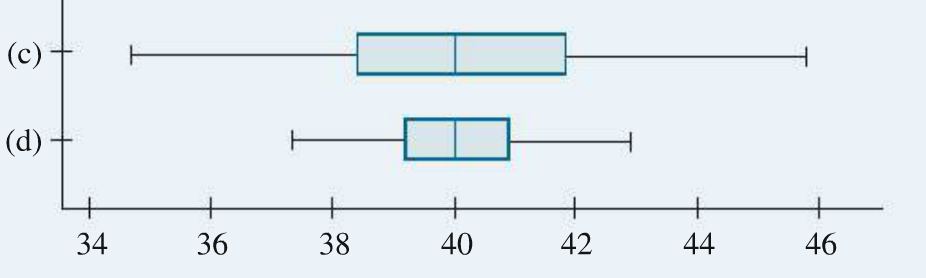
\includegraphics[scale=0.75]{Boxplots}
%\end{center}
%
%\newpage
%\noindent
%\section*{Announcements}
%\textbf{Tonight}
%\begin{itemize}
%	\item MyMathLab Section 4.2 due at 11:30pm
%\end{itemize}
%
%\textbf{Thursday, February 8}
%\begin{itemize}
%	\item Quiz 2 in class \textbf{bring your laptop}
%	\item MyMathLab Section 4.3 due at 11:30pm
%\end{itemize}
%
%\textbf{Sunday, February 11}
%\begin{itemize}
%	\item MyMathLab Review 1 due at 11:30pm
%\end{itemize}
%
%\textbf{Thursday, February 15}
%\begin{itemize}
%	\item \textbf{Exam 1} in class
%		\begin{itemize}
%			\item Pen or Pencil with dark lead
%			\item Calculator
%			\item Catcard
%		\end{itemize}
%\end{itemize}

%%%%%%%%%%%%%%%%%%%% Day 9 %%%%%%%%%%%%%%%%%%%%

%\noindent
%%The following histograms represent the daily high temperatures in San Mateo, California in May of 2014.
%
%%\begin{center}
%%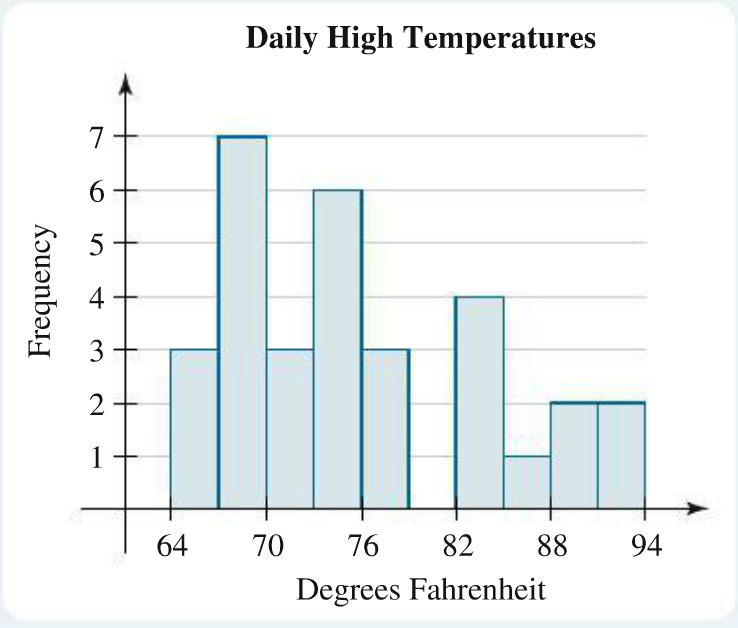
\includegraphics[scale=1]{bimodaltemps}
%%\end{center}
%%
%%\begin{center}
%%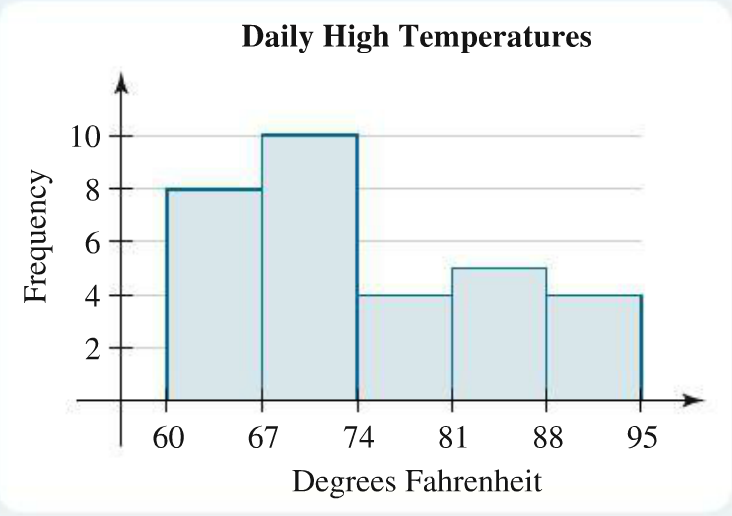
\includegraphics[scale=1]{unimodaltemps}
%%\end{center}
%
%\noindent
%Use these to answer the following questions:
%\begin{enumerate}
%	\item In San Mateo, there tend to be foggy days, and sunny days. Which of these histograms better represents this?
%	\item A person who doesn't like heat is looking into moving to San Mateo, which histogram would be better to show this person?
%	\item What is the difference between the two histograms?
%	\item Would you say that one of these graphs is misleading? How is it misleading?
%\end{enumerate}
%
%\newpage
%%\noindent
%%The following chart represents the annual revenue in billions of dollars of Nike.
%%
%%\begin{center}
%%	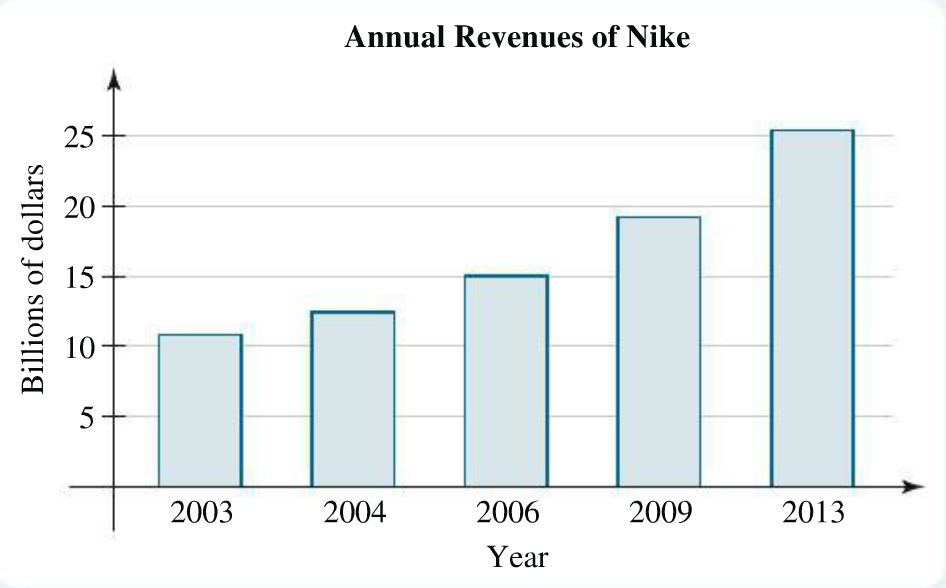
\includegraphics[scale=1]{Nikemisleading}
%%\end{center} 
%
%\noindent
%Use this graph to answer the following questions.
%\begin{enumerate}
%	\item Based on the graph what would you say about Nike's annual revenue?
%	\item What makes this graph misleading?
%	\item How could you fix it?
%\end{enumerate}
%
%\newpage
%\noindent
%%The following bar graph represents wine consumptions of several different countries.
%%
%%\begin{center}
%%	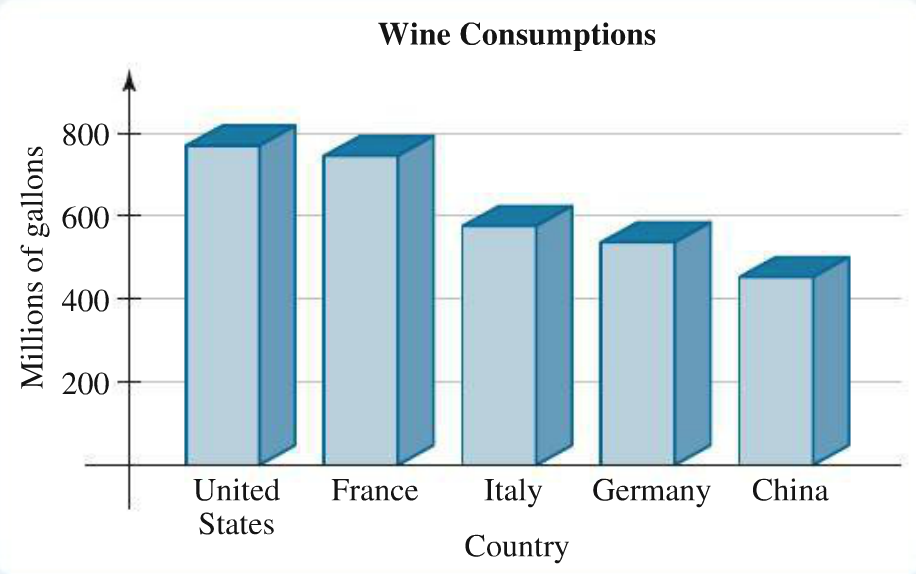
\includegraphics[scale=1]{3DMisleading}
%%\end{center}
%
%Use this graph to answer the following questions:
%\begin{enumerate}
%	\item Based on the graph which country consumes the most wine?
%	\item What makes this graph misleading?
%	\item How could we fix that problem?
%	\item In addition to the graph being misleading, the data presentation is misleading. What is something about the data presentation that is misleading?
%\end{enumerate}
%
%\newpage
%\noindent
%%The following Time Series Plots represent the United States market shares as a percentage or world manufacturing.
%%
%%\begin{center}
%%  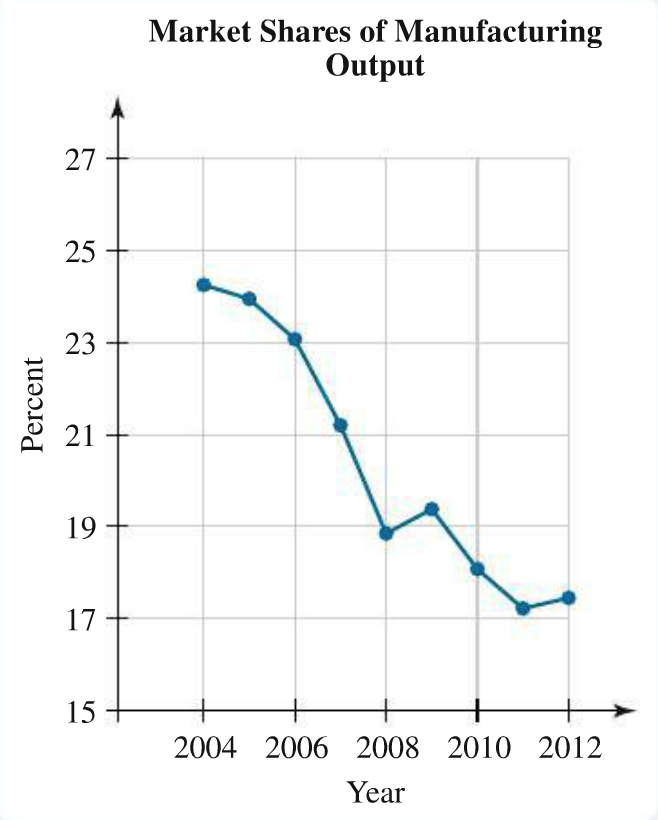
\includegraphics[scale=0.85]{Timeseriesmessedscale}
%%\end{center}
%%
%%\begin{center}
%%  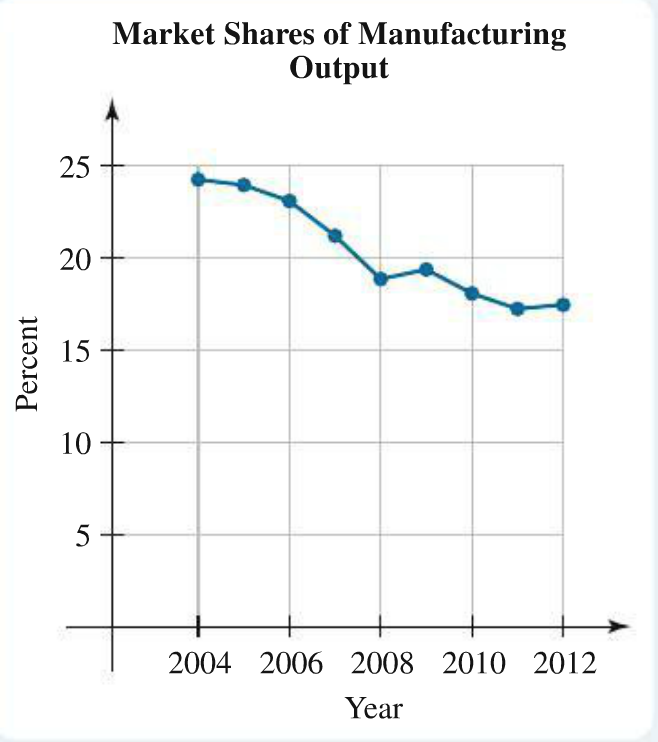
\includegraphics[scale=0.85]{Timeseriesregularscale}
%%\end{center}
%
%Use these to answer the following questions:
%\begin{enumerate}
%	\item How could the Republican party utilized one of these charts for the 2012 reelection season?
%	\item How could the Democratic party utilized one of these charts for the 2012 reelection season?
%	\item What is the difference between the two time series graphs?
%	\item Would you say that one of these graphs is misleading? How is it misleading?
%\end{enumerate}

%%%%%%%%%%%%%%%%%%%% Day 10 %%%%%%%%%%%%%%%%%%%%

%\section*{Warm-Up}
%Copy the following questions into your notes and then answer the questions.
%\begin{enumerate}
%	\item Is a frequency table used for categorical or numerical data?
%	\item What is an example of a discrete variable? $\ldots$ a numerical variable?
%	\item Do relative frequencies add up to 1 Sometimes? Always? Never?
%	\item Which is bigger? The number of female students at the UA \textbf{\underline{AND}} Female or the number of female students at the UA \textbf{\underline{OR}} Female? How do you know?
%	\item A histogram has 5 classes of class width 3, starting at 14. Write out all the classes.
%	\item Is the 50th percentile the same as the mean? Median? or Neither?
%	\item In a skewed left distribution, which is bigger $\overline{x}$ or $M$?
%	\item In a typical unimodal symmetric distribution, is the more data between $Q_1$ and $Q_3$ or within one standard deviation of the mean?
%\end{enumerate}

%%%%%%%%%%%%%%%%%%%% Day 12 %%%%%%%%%%%%%%%%%%%%

%\section*{Warm-Up} 
%Complete the following activities at your table.
%
%\noindent
%\begin{enumerate}
%	\item Designate a person at your table to be Player A and a person to be Player B
%	\item Play 20 games of Rock/Paper/Scissors at your table and record who won on your white board after each game. (Make sure to establish the rules with which you will play first)
%	\item Use the results to answer the following questions:
%		\begin{enumerate}
%			\item What proportion of times did Player A win?
%			\item What proportion of times did Player B win?
%			\item List all possible outcomes for each round. (i.e. RR for rock and rock)
%			\item Is the game ``fair"? Why or why not?
%		\end{enumerate} 
%\end{enumerate}
%
%\newpage
%\noindent
%Think about the Rock Paper Scissors Example we started with at the beginning of class. Use that to answer the following questions:
%\begin{enumerate}
%	\item What is the sample space? \vspace{3cm}
%	\item What does the event A wins contain? \vspace{3cm}
%	\item What is P(A wins)? \vspace{2.5cm}
%	\item What is P(B wins)? \vspace{2.5cm}
%	\item What is P(Tie)? \vspace{2.5cm}
%	\item Is it more likely that someone wins or there is a tie?
%	\item Is the game fair? \vspace{2.5cm}
%\end{enumerate}
%
%\newpage
%\noindent
%List/Describe the sample spaces for the following experiments:
%\begin{itemize}
%	\item Drawing a card from a deck of cards \vspace{2.5cm}
%	\item Rolling a 20 sided dice \vspace{2.5cm}
%	\item Flipping a coin 3 times
%\end{itemize}
%
%
%\newpage
%\noindent
%\begin{center}
%	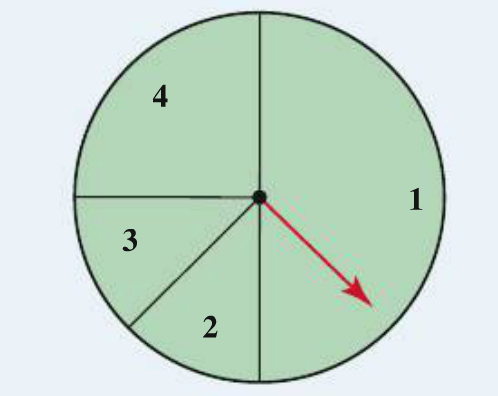
\includegraphics[scale=1.5]{Spinner}
%\end{center}
%Use the spinner to answer the following questions:
%\begin{enumerate}
%	\item Are all outcomes equally likely?\vspace{2.5cm}
%	\item Give an example of a sure event. \vspace{2.5cm}
%	\item Given an example of an impossible event. \vspace{2.5cm}
%	\item Find $P(X=4)$, $P(X\leq 2)$ and $P(\text{at least } 2)$ 
%\end{enumerate}
%
%\newpage
%\noindent
%Consider rolling a six-sided dice once. Answer the following questions:
%\begin{enumerate}
%	\item What is the sample space?
%	\item Are the outcomes equally likely?
%	\item Give an example of a sure event.
%	\item Give an example of an impossible event.
%	\item Find $P(X=2)$
%	\item Find $P(3 \leq X \leq 6)$ 
%	\item Find $P(\text{at most } 4)$
%	\item Find $P(2<X<5)$
%\end{enumerate}

%%%%%%%%%%%%%%%%%%%% Test Waiver %%%%%%%%%%%%%%%%%%%%

%\noindent
%By signing this document I, \underline{\hspace{7.5cm}}, acknowledge the following:
%\begin{itemize}
%	\item I am taking Exam 1 for Math 107 on Wednesday, February 21, 2018 at 3pm. 
%	\item The exam was originally scheduled for Thursday, February 15, 2018 at 8am.
%	\item I did not contact my instructor before the exam stating that I would not be in class that day.
%	\item I will be assessed a 10\% penalty for taking the exam late. 
%\end{itemize} 
%
%\vspace{1.5cm}
%
%\noindent
%Name: \underline{\hspace{7.5cm}}\\ \vspace{1.5cm}
%
%\noindent
%Signature: \underline{\hspace{7.5cm}}\\ \vspace{1.5cm}
%
%\noindent
%Date: \underline{\hspace{5cm}}

%%%%%%%%%%%%%%%%%%%% Day 13 %%%%%%%%%%%%%%%%%%%%

%\begin{enumerate}
%	\item 25.45\% of the students in our class are majoring in Political Science. Use this to answer the following questions:
%	\begin{enumerate} 
%	\item What is the probability that if we were to select a random student from our class that they are a political science major?
%	\item What is the probability that if we were to select a random student from our class that they are \textbf{NOT} a political science major?
%	\end{enumerate}
%	\item 60\% of the students in our class our freshman. What is the probability that if we were to select a random student from the class they are \textbf{NOT} a freshman?
%	\item Based on the previous two questions, what sort of rule can you come up with to calculate the probability of an event \textbf{NOT} happening?
%\end{enumerate}
%
%\newpage
%
%\begin{problem}{}
%Use the following pie chart regarding a survey conducted about social medias influence on purchasing decisions to answer some questions.
%\begin{center}
%	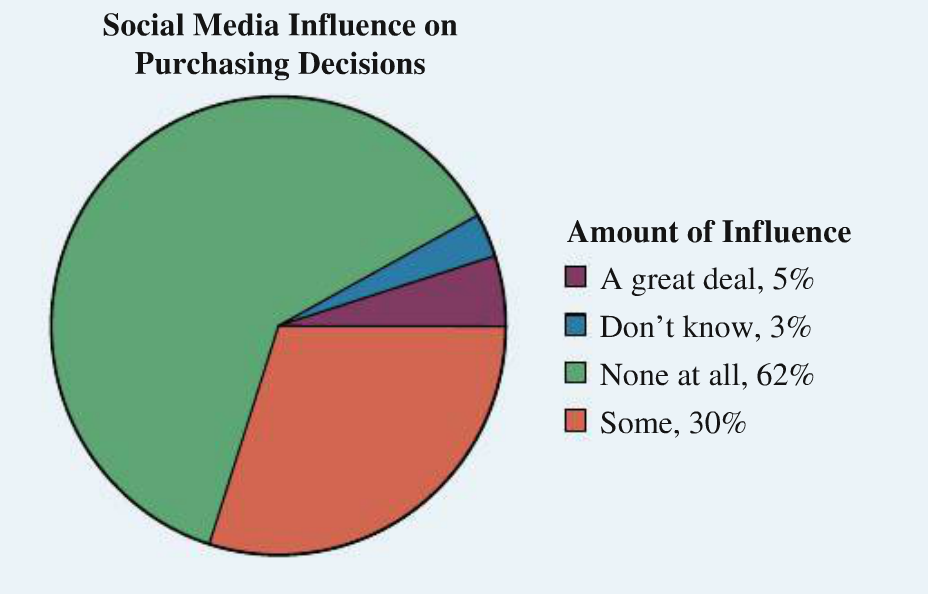
\includegraphics[scale=0.75]{Piechartforprobpractice}
%\end{center}	
%\noindent
%Let $N$ be the event None at all and $S$ be the event some.
%\begin{enumerate}[label=\rm{(\alph*)}]
%	\item Find $P(N)$
%	\item Find $P(S)$
%	\item What is $P( N \textbf{ OR } S)$?
%	\item What is $P( \textbf{NOT } S)?$
%	\item From inspecting the data a student concludes that 62\% of all American adults think that social media has no impact on their purchasing demands. What would you tell this student?
%\end{enumerate}
%\end{problem}
%
%\newpage
%
%\begin{problem}
%	Use the following chart to answer some questions about probability.
%	\begin{center}
%		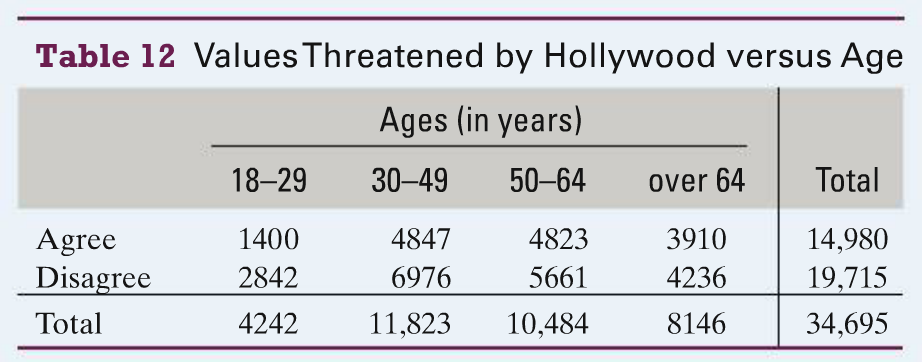
\includegraphics[scale=1]{Probpractice}
%	\end{center}
%	Let $A$ be the event Agree, $T$ be the event 18 -- 29, $F$ be the event 50 -- 64.
%	\begin{enumerate}[label=\rm{(\alph*)}]
%		\item Find P(A)
%		\item Find P(A \textbf{OR } T)
%		\item Find P(\textbf{NOT } F)
%		\item Find P(A \textbf{AND} T)
%	\end{enumerate}
%\end{problem}
%
%\newpage
%
%\begin{problem}
%	\item Think of two events that are mutually exclusive.
%	\item Think of two events that are disjoint.
%	\item Think of two events that are not disjoint.	
%\end{problem}

%%%%%%%%%%%%%%%%%%% Day 14 %%%%%%%%%%%%%%%%%%%

%\noindent
%Several semesters ago, Candace and Zach were taking SBS 200 in the same semester. On their first exam Candace scored a 66.4 out of 83 points and Zach scored a 268.8 out of 336. Candace claims that she did better on the exam than Zach but Zach disagrees. Who scored better on Test 1? How do you know?\\
%
%\newpage
%\noindent
%Not to be deterred Candace and Zach both talked to their instructors and found that the data for their exams was symmetric and unimodal. Candace found out that her class had a mean of 61 and a standard deviation of 6. Zach found out that his class had a mean of 254 and a standard deviation of 10. Use this information to answer the following questions:
%
%\begin{enumerate}
%	\item Which test was harder? How do you know?
%	\item Did Candace score within one standard deviation of the mean? Did Zach? How do you know?
%	\item Did Candace score within two standard deviations of the mean? Did Zach? How do you know?
%	\item Did Candace score within 3 standard deviations of the mean? Did Zach? How do you know?
%	\item How many standard deviations above the mean did Candace score?\\ How many standard deviations above the mean did Zach score?
%	\item Who did better on the exam?
%\end{enumerate}
%
%\newpage
%\noindent
%Assume that all of the following data sets are normally distributed. Calculate and interpret the $z$-score for the following scenarios: 
%\begin{enumerate}
%	\item Observations: The lengths of songs, in seconds,  played on \textit{Live 105} on April 18, 2014\\ $\overline{x}=232.92$\\ $s=46.93$\\ Coldplay song of 285 seconds
%	\item Observations: Temperature at the top of every hour in February 2014 in Tucson, Arizona\\ $\overline{x}=64.6^{\circ}F$\\ $s=12.2^{\circ}F$\\ The coldest observed temperature of $27^{\circ}F$
%	\item Observations: IQ scores\\ $\overline{x}=100$\\ $s=15$\\ Kim Ung-yong, a Korean child prodigy has an IQ score of 210
%	\item Observations: IQ scores\\ $\overline{x}=100$\\ $s-15$\\ The $z-$score of George Washington is estimated to be 2.167 and the $z-$score of Abraham Lincoln is estimated to be 2.667. What are their corresponding IQ's?
%\end{enumerate}
%
%\newpage
%\noindent
%\begin{enumerate}
%	\item What does it mean to have a $z$-score of 0?
%	\item What is the probability that a random observation has a negative $z$-score?
%	\item What is the probability that a random observation has a positive $z$-score?
%	\item What is $P(-1 <z<1)$?
%	\item What is $P(-2<z<2)$?
%	\item What is $P(-3<z<3)$?
%\end{enumerate}

%%%%%%%%%%%%%%%%%%% Day 15 %%%%%%%%%%%%%%%%%%%

%\noindent
%What is the probability that a randomly selected observation from a collection of normally distributed data that a $z$-score is less than 1? \\ \vspace{3.5cm}
%
%\noindent
%Answer the following questions with your group regarding $z$-scores:
%\begin{enumerate}
%	\item $P(z<1.22)$
%	\item $P(z>1.22)$
%	\item $P(z<-0.45)$
%	\item $P(-0.45<z<1.22)$
%	\item $P(z<-0.45 \textbf{ OR } z>1.22)$
%\end{enumerate}
%
%\newpage
%\begin{enumerate}
%	\item Observations: The lengths of songs, in seconds,  played on \textit{Live 105} on April 18, 2014\\ $\overline{x}=232.92$\\ $s=46.93$\\ What is the probability that you tuned into the radio and listened to a song that is 220 seconds long?
%	\item Observations: Temperature at the top of every hour in February 2014 in Tucson, Arizona\\ $\overline{x}=64.6^{\circ}F$\\ $s=12.2^{\circ}F$\\ What is the probability that you experienced a temperature that was greater than $36^{\circ}$?
%	\item Observations: IQ scores\\ $\overline{x}=100$\\ $s=15$\\ Nicole Kidman has  an IQ of 132 and Shakira has an IQ of 140. What is the probability that if we were to pick a random person they would have an IQ score between 132 and 140?
%\end{enumerate} 
%
%\newpage
%\begin{enumerate}
%	\item A pizza restaurant claims that its mean deliver time is 30 minutes with a standard deviation of 4. An undercover shopper times the amount of time it takes to get her pizza delivered which takes 40 minutes. Is the 40 minute delivery an unusual event?
%	\item For students that graduated high school in 2017 had a mean combined score of  1060 and a standard deviation of 195. Jacque a freshman this year had a combined score of 1320. Is this an unusual score? What is Jacque's percentile?
%	\item For students that graduated high school in 2017 had a mean combined score of  1509 and a standard deviation of 102. Eloise, graduated in 2010 this year had a combined score of 1680. Is this an unusual score? What is Eloise's percentile?
%	\item Using the two questions above what is the probability that a randomly selected student from last years graduating class had a score between Jacque and Eloise?
%\end{enumerate}
%
%\newpage
%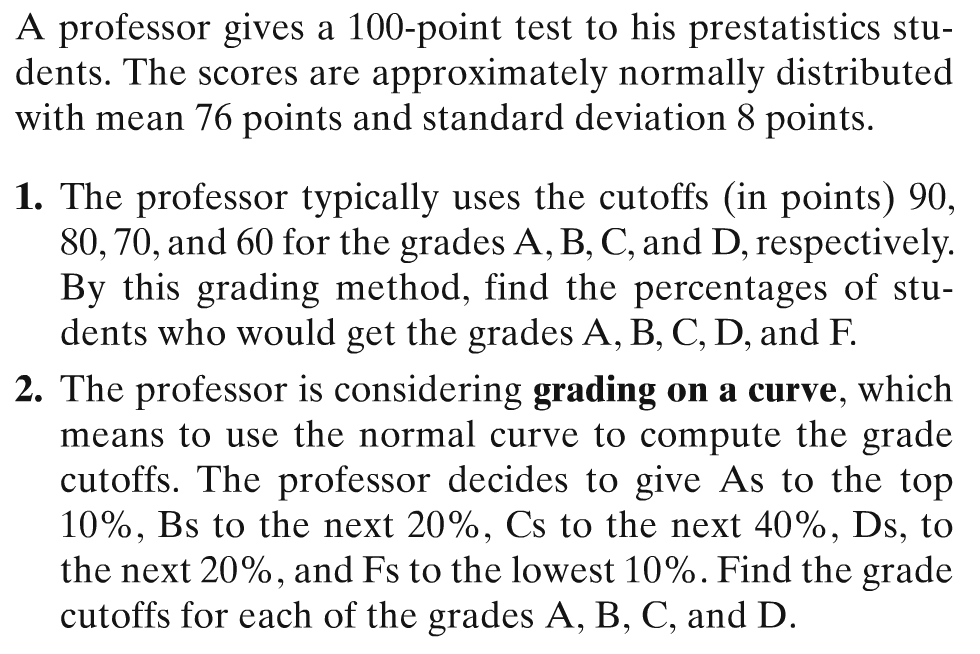
\includegraphics{Gradeonacurve1}
%
%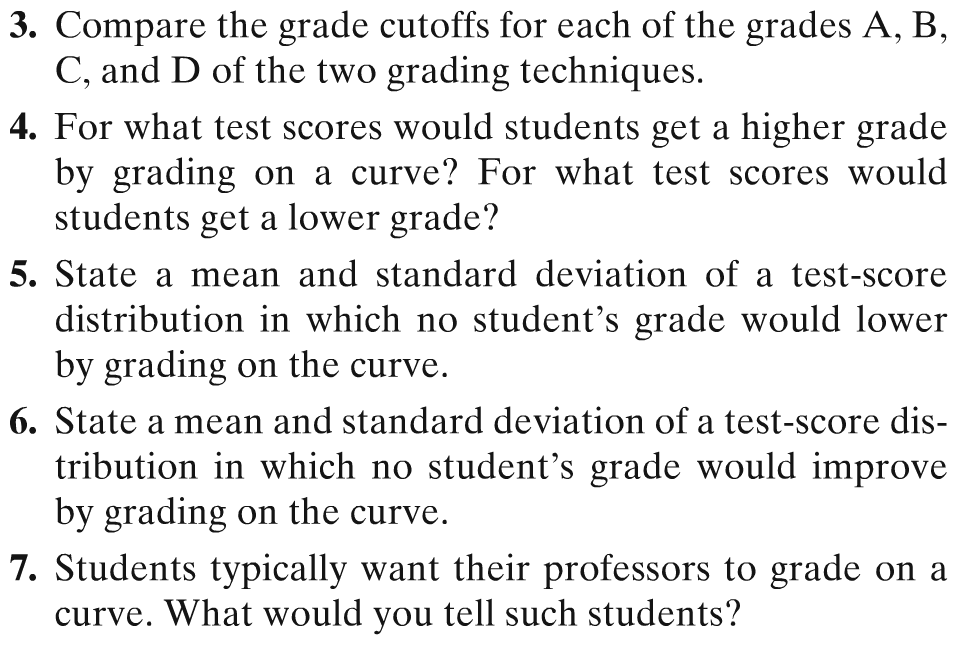
\includegraphics{Gradeonacurve2}


%%%%%%%%%%%%%%%%%%% Day 16 %%%%%%%%%%%%%%%%%%%

%\section*{Warm-up}
%\begin{enumerate}
%	\item The $z$-score of an observation is the number of \underline{\hspace{2.5cm}}.
%	\item The $z$-score of an observation $x$ is found by $z=$\underline{\hspace{2.5cm}}, where $\overline{x}$ is \underline{\hspace{2.5cm}} and $s$ is \underline{\hspace{2.5cm}}.
%	\item A professor recently gave a test to his students and the results were approximately normally distributed. The test had a mean of 70 and a standard deviation of 12.5. 
%		\begin{enumerate}
%			\item Cameron received a score that corresponds to a $z$-score of 2. What score did she get on the test?
%			\item Cameron claims her grade places her in the 97th percentile of all grades on the test. Do you agree or disagree with her? Why?
%			\item Cameron's friend Colin recently took a test over the same material but his section had an average of 78 and a standard deviation of 5. Colin received a score that corresponded to a $z$-score of -1. What grade did he get on the test? 
%			\item Approximately what percent of students had a lower grade than Colin?
%			\item On the same x-axis draw a normal curve that represents the results for Cameron's test and a normal curve that represents the results for Colin's test.
%			\item Compare the two curves. 
%			\item How is the normal curve affected by the mean?
%			\item How is the normal curve affected by standard deviation?
%		\end{enumerate}
%\end{enumerate}
%
%\newpage
%\noindent
%In the Fuel Economy Guide for 2014 model vehicles completed by the Environmental Protection Agency (EPA) published that the combined city and highway gas mileage for non-hybrid vehicles is approximately normally distributed with a mean of 22.2 miles per gallon and a standard deviation of 5.2 mpg. Use this to answer the following questions.
%\begin{enumerate}
%	\item The 2014 Volkswagen Beetle has a combined gas mileage of 28 mpg. What percent of all vehicles have worse gas mileage than the Beetle?
%	\item The 2014 Ford F-150 has a combined gas mileage of 20 mpg. What percentage of all vehicles have better gas mileage than the Ford F-150?
%	\item To receive an award for fuel efficiency a vehicle must be in the top 5\% of all vehicles. What must the gas mileage of a vehicle be in order to fall in the top 5\% and receive an award?
%	\item The EPA did not include hybrid vehicles in the normal curve. Why did they not include these vehicles?
%\end{enumerate}
%
%\newpage
%\noindent
%A professor gave a test worth 100 points. The results were normally distributed with a mean of 70 and a standard deviation of 10. Use this information to answer the following questions.
%\begin{enumerate}
%	\item Complete the following table: \begin{center}
%		\begin{tabular}{|l|l|l|l|}
%\hline
%Grade & Cutoff & \% of students with this grade & z-score \\ \hline
%A     & 90     &                                &         \\ \hline
%B     & 80     &                                &         \\ \hline
%C     & 70     &                                &         \\ \hline
%D     & 60     &                                &         \\ \hline
%F     & -      &                                &         \\ \hline
%\end{tabular}
%	\end{center}
%	\item The professor is considering grading on a curve. He will give the grades based on the following table. Complete this table: \begin{tabular}{|l|l|l|l|}
%\hline
%Grade & Cutoff & \% of students with this grade & z-score \\ \hline
%A     &        & 10                             &         \\ \hline
%B     &        & 20                             &         \\ \hline
%C     &        & 40                             &         \\ \hline
%D     &        & 20                             &         \\ \hline
%F     &        & 10                             &         \\ \hline
%\end{tabular}
%	\item  Comparing the two tables answer the following questions:
%		\begin{enumerate}
%			\item For which test scores would a student get a higher grade on the test?
%			\item For which test scores would a student get a lower grade on the test?
%			\item Student's typically want their professors to grade on a curve. What would you tell these students? 
%		\end{enumerate}
%\end{enumerate}

%%%%%%%%%%%%%%%%%%% Day 20 %%%%%%%%%%%%%%%%%%%
%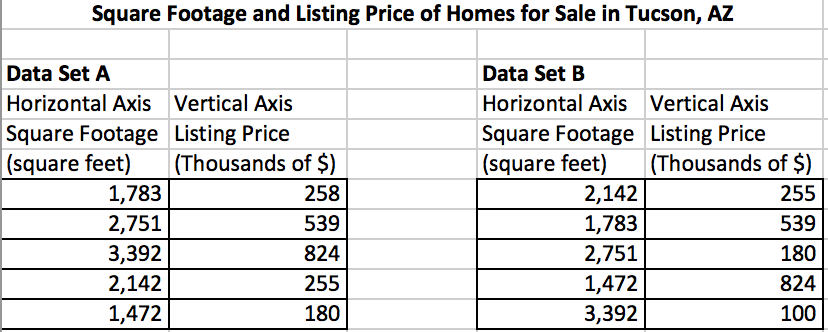
\includegraphics{HousingPricesTucson}\\
%Use the above data set to do the following:
%\begin{itemize}
%	\item Take out two whiteboards and on each draw a set of coordinate axes that have a horizontal axis that starts at 0 and increases to 4,000 with marks at every 500 and a vertical axis that starts at 0 and increases to 900 with ticks at every 100. 
%	\item On one set of axes plot the points of Data Set A
%	\item On the other set of axes plot the points of Data Set B
%\end{itemize}
%
%\begin{enumerate}
%	\item One of the data sets is real, and the other is made up. Based on your plots which one do you think is real? Why?
%	\item Do you think a 2,500 square foot home in Tucson is on sale for \$400,000 currently? If not, what would be a reasonable price for such a house?
%	\item A relator listed a 3,000 square foot home for \$100,000 recently. Give three possible reasons that might explain this data point.
%\end{enumerate}

%%%%%%%%%%%%%%%%%%% Day 21 %%%%%%%%%%%%%%%%%%%

%\subsection*{Warm-up Question}
%The following table represents the overdraft fees collected by banks in certain years since 2000. 
%\begin{center}
%\begin{tabular}{c|c}
%Year & \begin{tabular}[c]{@{}l@{}}Amount of Overdraft Fees\\ (billions of dollars)\end{tabular} \\
%2001 & 22.2                                                                                     \\ \hline
%2003 & 27.1                                                                                     \\ \hline
%2005 & 29.7                                                                                     \\ \hline
%2007 & 34.1                                                                                     \\ \hline
%2009 & 37.1                                                                                    
%\end{tabular}
%\end{center}
%Let $A$ be the total amount (in billions of dollars) of overdraft fees collected in the year that is $t$ years since 2000. Using the whiteboards at your table answer the following questions.
%\begin{enumerate}
%	\item Construct a scatterplot (if you use your calculator make sure to draw a sketch of it)
%	\item Draw a (straight) line that comes close to all of the data points in your scatterplot.
%	\item Use your line to estimate the total amount of fees collected in 2008.
%	\item Use your line to estimate when the total amount of fees collected was \$32 billion.
%	\item Find the point where the line intersects the $A$-axis. What does it mean in this situation?
%	\item Use your line to estimate the total amount of fees collected in 2011. Compare your result with \$31.6 billion, which is the actual amount. 
%\end{enumerate}
%
%\newpage
%\noindent
%The percentages of cell phone users who send or receive text messages multiple times per day are shown for various ages.\\
%
%\begin{center}
%	\begin{tabular}{c|c}
%Age ($a$)  & Percent ($p$) \\ \hline
%21   & 76      \\ \hline
%29.5 & 63      \\ \hline
%39.5 & 42      \\ \hline
%49.5 & 37      \\ \hline
%59.5 & 17     
%\end{tabular}
%\end{center}
%
%\begin{enumerate}
%	\item Determine the explanatory variable and the response variable.
%	\item Draw a scatterplot that represents the data. 
%	\item Describe the shape, association and direction of the association.
%	\item Draw a linear model that fits the data.
%	\item Predict the percentage of 35-year-old cell phone users who send or receive text messages multiple times per day. 
%	\item Find where the graph crosses through the $p$-axis. In context of the problem, what does this mean?
%	\item Find where the graph crosses through the $a$-axis. In context of the problem what does this mean?
%\end{enumerate}
%
%\newpage
%\noindent
%The following represents the number of collisions at highway-railroad crossings per year since 1990.
%\begin{center}
%	\begin{tabular}{ll}
%Year & Number of Collisions \\
%1992 & 4.9                  \\
%1995 & 4.6                  \\
%2000 & 3.5                  \\
%2005 & 3.1                  \\
%2010 & 2.1                  \\
%2014 & 2.3                 
%\end{tabular}
%\end{center} 
%
%\begin{enumerate}
%	\item Determine which variable is the explanatory variable, and which is the response variable.
%	\item Draw a scatterplot that represents the situation.
%	\item Describe the four characteristics of the association.
%	\item Draw a linear model on your scatter plot.
%	\item Use your model to predict the number of collisions in 2012. Did you perform interpolation or extrapolation?
%	\item Use your model to predict the number of collisions will be 1.0 thousand. 
%	\item Do you have faith in your result? Why or why not?
%	\item Find the $t$-intercept. What does it mean in this situation?
%	\item Do you have faith in your result? Why or why not?
%\end{enumerate}

%%%%%%%%%%%%%%%%%%% Day 22 %%%%%%%%%%%%%%%%%%%

%\noindent
%Paul and Judy did some baking this past weekend. At 1 pm Paul realized he forgot to preheat the oven and immediately turned it on. His oven was $75^{\circ}$F and the temperature began to rise $50^{\circ}$F per minute. Judy on the other hand preheated her oven so that at 1pm her oven was $375^{\circ}$F and stayed at this temperature. 
%\begin{enumerate}
%	\item Make a table that represents Paul and Judy's oven temperature for every minute between 1pm and 1:10pm.
%	\item Make a scatterplot for Paul's oven temperature from 1pm to 1:10pm.
%	\item On the same set of axes make a scatterplot for Judy's oven temperature.
%	\item Draw a linear model for Paul's oven temperature.
%	\item How would you describe the association of Paul's oven temperature?
%	\item Using you linear model, estimate when Paul's oven was the same temperature as Judy's oven.
%\end{enumerate}
%
%\newpage
%\noindent
%\begin{enumerate}
%	\item Find four solutions to the equation $y=-2x+6$ and find four points that do not satisfy the equation.
%	\item On a coordinate axis draw all 8 points and draw the graph of the equation $y=-2x+6$
%	\item Find the $x$ and $y$ intercepts of the equation and label them on your graph.
%	\item Repeat Parts 1 -- 3 from above for the equations $y=2x-2$.
%\end{enumerate}
%
%\newpage
%\noindent
%Erin Gilbert recorded the number of calls, $N$, the Ghostbusters received over several evenings when the temperature is, $T$, in degrees celsius. The following is what she recorded:
%
%\begin{center}
%	\begin{tabular}{l|lllllll}
%$T$ & 19 & 27 & 21 & 15 & 23 & 11 & 14 \\ \hline
%$N$ & 29 & 13 & 24 & 33 & 18 & 44 & 36
%\end{tabular}
%\end{center}
%
%\begin{enumerate}
%	\item Decide on the explanatory/response variables and \textit{carefully} plot the data.
%	\item Is the association positive, negative or neither.
%	\item Graph the line $y=-2x+63$ on the same set of axes. Does the line come close to the data points.
%	\item Find the $x$ and $y$ intercepts of the equation. In the context of the problem what do they mean?
%\end{enumerate}


%%%%%%%%%%%%%%%%%%% Day 23 %%%%%%%%%%%%%%%%%%%

%\noindent
%Alfredo works on campus in Residence Life as a desk assistant. For the past few paychecks the he has been keeping track of the amount of money he has earned. The following table summarizes the results: 
%\begin{center}
%	\begin{tabular}{c|c}
%Number of Hours & Paycheck Amount \\ \hline
%20              & \$200           \\
%12.5            & \$125           \\
%9.25            & \$92.5          \\
%10              & \$100          
%\end{tabular}
%\end{center}
%
%\begin{enumerate}
%	\item Draw a scatterplot that represents this situation.
%	\item Identify the 4 characteristics of association
%	\item Find the rate of change between 4 pairs of data points.
%	\item Compare the rates of change you calculated (how are they similar, how are they different)
%\end{enumerate}
%
%\newpage
%
%\noindent
%The numbers in thousands of service members in the armed forces diagnosed as overweight for various years is shown below.
%
%\begin{center}
%	\begin{tabular}{c|c}
%Years & Number of Overweight Service Members \\ \hline
%2006  & 56                                   \\
%2007  & 62                                   \\
%2008  & 72                                   \\
%2009  & 29                                   \\
%2010  & 86                                  
%\end{tabular}
%\end{center}
%
%\hspace{4cm}
%
%\begin{enumerate}
%	\item Draw a scatterplot that represents this situation.
%	\item Identify the 4 characteristics of association
%	\item Find the rate of change between 4 pairs of data points.
%	\item Compare the rates of change you calculated (how are they similar, how are they different)
%\end{enumerate}
%
%\hspace{7cm}
%
%\noindent
%\textbf{Use the examples from above to answer the following questions:}
%\begin{enumerate}
%	\item Compare the two data sets. How are they similar? How are they different?
%	\item Make a generalization about the relationship between $r$-values and the rate of change for a linear model.
%\end{enumerate}
%
%
%\newpage
%
%\begin{problem}
%The volume of water in a swimming pool increases steadily by 2400 gallons in an 8-hour period. Find the rate of change of volume of water.
%\end{problem}
%
%
%\begin{problem}
%	The temperature decreases steadily by $15^\circ$F over a 3-hour period. Find the rate of change of temperature.
%\end{problem}
%
%\vspace{7cm}
%
%\begin{problem}
%	The number of female-owned firms increased approximately steadily from 5.4 million firms in 1997 to 8.6 million firms in 2013. Find the approximate rate of change of the number of female-owned firms.
%\end{problem}
%
%\begin{problem}
%	The number of U.S. cable TV subscribers decreased approximately steadily from 61.8 million subscribers in 2009 to 54.3 million subscribers in 2014. Find the approximate rate of change of the number of U.S. cable TV subscribers.
%\end{problem}
%
%\newpage
%
%\begin{problem}
%	The scatterplot and the linear model below describe the association between years and the numbers (in millions) of Americans without health insurance.
%	\begin{center}
%		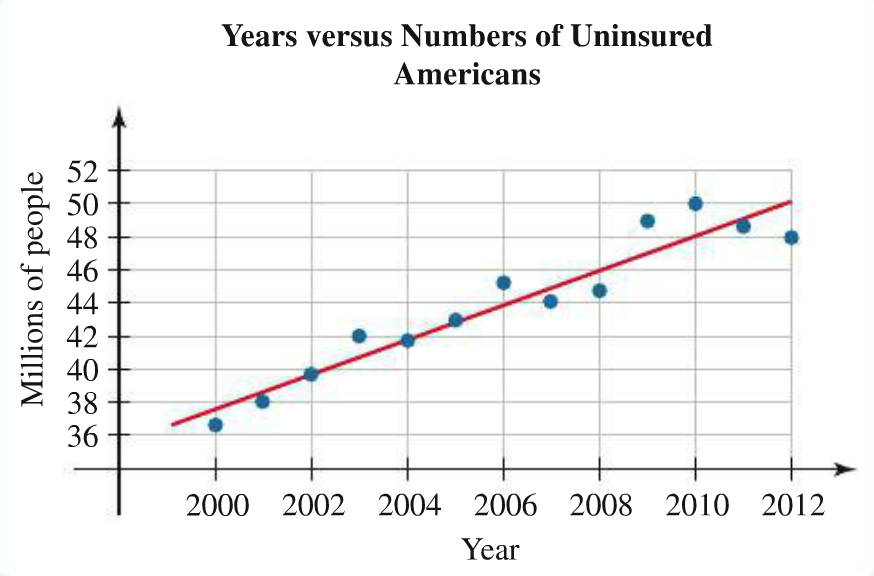
\includegraphics[scale=0.65]{insurance}
%	\end{center}
%	\begin{itemize}
%		\item Describe the direction of the association. What does it mean in the context of the problem?
%		\item Estimate the rate of change of the number of Americans without health insurance.
%	\end{itemize}
%\end{problem}
%
%\begin{problem}
%	The scatterplot and the linear model below describe the association between years and women's 200 meter run record times in seconds.
%	\begin{center}
%		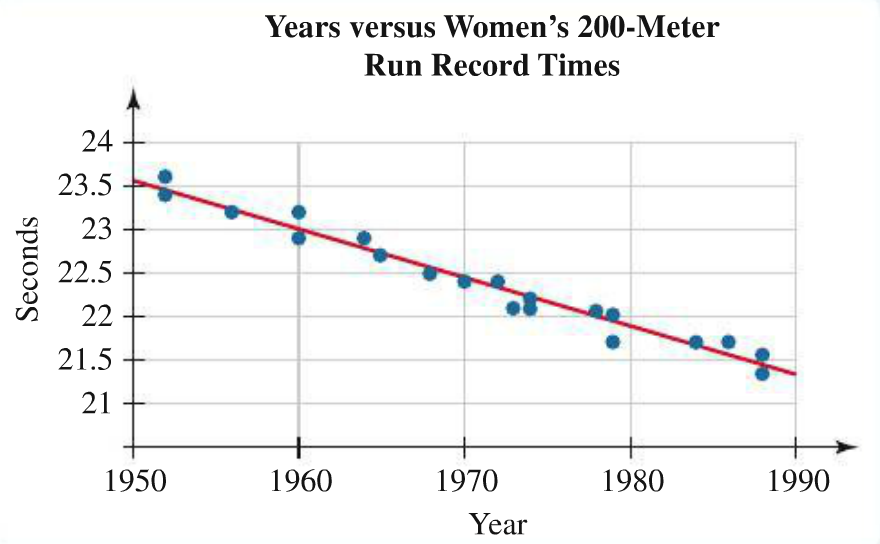
\includegraphics[scale=0.65]{run}
%	\end{center}
%	\begin{itemize}
%		\item Describe the direction of the association. What does it mean in the context of the problem?
%		\item Estimate the rate of change of the number of Americans without health insurance.
%	\end{itemize}
%\end{problem}

%%%%%%%%%%%%%%%%%%% Day 24 %%%%%%%%%%%%%%%%%%%

%Amazon.com's revenues are show below for several years.
%\begin{center}
%	\begin{tabular}{c|c}
%Year & \begin{tabular}[c]{@{}c@{}}Revenue\\ (billions of dollars)\end{tabular} \\ \hline
%2010 & 34.2                                                                    \\
%2011 & 48.1                                                                    \\
%2012 & 61.1                                                                    \\
%2013 & 74.5                                                                    \\
%2014 & 89.0                                                                   
%\end{tabular}
%\end{center}
%
%\noindent
%Define revenue to be $r$ and $t$ to be years since 2010. Use this data and information to answer the following questions:
%\begin{enumerate}
%	\item Create a scatterplot to represent the data on the whiteboard and on your graphing calculator.
%	\item Describe the 4 characteristics of association for this data.
%	\item Calculate the rate of change between 2010-2011, 2012-2014 and 2010-2014.
%	\item A linear model that represents this data is given by $r=13.6t+34.18$. Use your graphing calculator to graph this line for directions using a TI calculator see A.16-A.18 in the text book for instructions on how to do this. Also sketch the line on your scatterplot you drew on the whiteboard.
%	\item Do you think this linear model is a good model for the situation? Why or why not?
%	\item Compare your answers of rate of change to the rate of change in the model. 
%	\item Use the model to predict the revenue in 2019. Did you perform interpolation or extrapolation? Do you have faith in your estimation?
%\end{enumerate}
%
%\newpage
%
%\begin{enumerate}
%	\item Graph $y=-x+2$ \\[5cm]
%	\item Graph $y=\frac{5}{2}x-3$ \newpage
%	\item Graph the line that has $m=\frac{2}{3}$ and passes through the point $(4,-5)$. \\[5cm]
%	\item Graph the line that has $m=\frac{-3}{4}$ and passes through the point $(6,3)$. \newpage
%	\item Graph the line that has $m=0$ and passes through the point $(2,3)$. \\[5cm]
%	\item Graph the line that has $m$ undefined and passes through the point $(1,4)$. \newpage
%	\item Graph the line $x=7$ \\[5cm]
%	\item Graph the line $y=3$ \newpage
%	\item Graph a line in which $m$ is positive and $b$ is negative. \\[5cm]
%	\item Graph a line in which $n$ is negative and $b$ is positive. \newpage
%\end{enumerate}
%
%
%\begin{enumerate}
%	\item Write an equation for the line that passes through $(0,-4)$ and $(1,7)$.\\[5cm]
%	\item Write an equation for the line that passes through $(0,3)$ and $(1,4)$. \newpage
%	\item Write an equation for the line that has the following graph:
%		\begin{center}
%			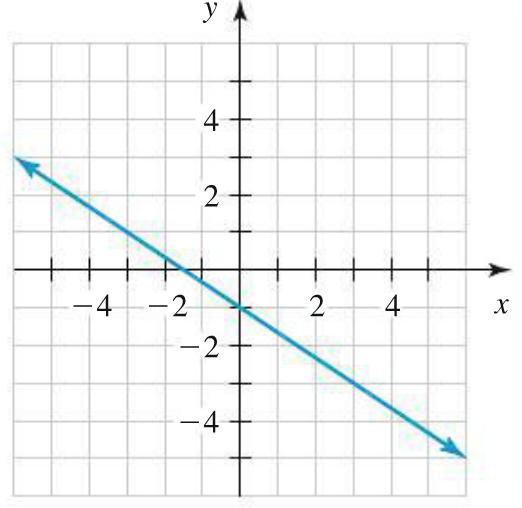
\includegraphics[]{negline} \\[5cm]
%		\end{center} 
%	\item Write an equation for the line that has the following graph:
%		\begin{center}
%			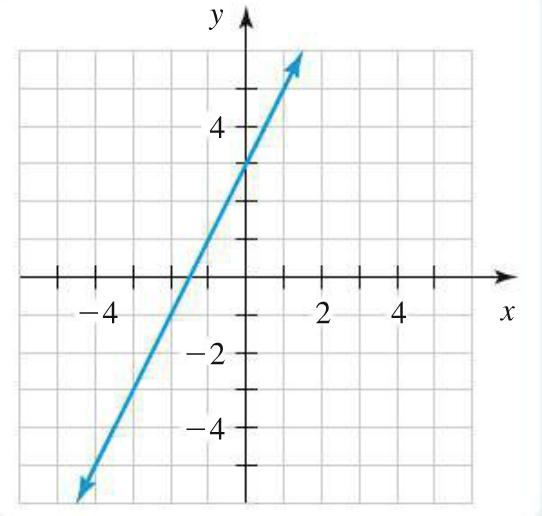
\includegraphics[]{posline}
%		\end{center}
%\end{enumerate}
%
%\newpage
%
%
%\begin{enumerate}
%	\item Let $n$ be the number of firefighters who died on duty in the year that is $t$ years since 2010. For the period 2010-2014, a reasonable model is $n=-2t+83$. Graph the model by hand. Estimate the number of firefighters who died in on duty in 2013. \\[5cm]
%	\item Let $H$ be the price (in dollars) or a hot dog, and let $S$ be the price (in dollars) of a soft drink both at a Major League Baseball stadium. For hot dog prices between \$1 and \$6.25, inclusive, a reasonable model is $S=0.8H+0.4$. Graph the model by hand. Predict the price of a hot dog at an MLB stadium where a soft drink costs \$4. \newpage
%	\item Google's revenue was \$29 billion in 2010, and it increased by about \$9 billion per year until 2014. Let $r$ be the annual revenue (in billions of dollars) at $t$ years since 2010.
%		\begin{itemize}
%			\item Identify the explanatory and response variables.
%			\item Find the slope and the $r$-intercept of a linear model.
%			\item Find an equation of the model.
%			\item Graph the model by hand
%			\item Estimate Google's revenue in 2014. \\[5cm]
%		\end{itemize}
%	\item A student's savings account has a balance of \$4,700 on September 1. Each month for 6 months, the balance declines by \$650. Let $B$ be the balance (in dollars) at $t$ months since September 1.
%		\begin{itemize}
%			\item Why is there a linear association between $t$ and $B$?
%			\item Find the slope of a linear model. What does it mean in this situation?
%			\item Find an equation of the model.
%			\item Graph the model by hand
%			\item When was the balance \$1450?
%		\end{itemize}
%\end{enumerate}
%
%\newpage
%\noindent
%Although the United States and Great Britain use the Fahrenheit temperature scale, most countries use the Celsius scale. The temperature reading $)^\circ$C is equivalent to the Fahrenheit reading $32^\circ$F. An increase of $1^\circ$C is equivalent to an increase of $1.8^\circ$F. Let $F$ be the Fahrenheit reading that is equivalent to a Celsius reading of $C$ degrees. Assume that $F$ is the response variable.
%\begin{enumerate}
%	\item Why is there an exact linear association?
%	\item What is the $F$-intercept of the model? What does it mean in this situation?
%	\item Find an equation of the model.
%	\item If the temperature is $30^\circ$C, what is the Fahrenheit reading?
%\end{enumerate}


%%%%%%%%%%%%%%%%%%% Day 28 %%%%%%%%%%%%%%%%%%%

%\begin{enumerate}
%	\item In 2000, 15 billion pounds of avocados were consumed. In 2014, 37 billion pounds were consumed. Find the rate of change in avocado consumption over this period.
%	\item Let $A$ be the annual U.S. consumption in billions of pounds of avocados at $t$ years since 2000. Which variable is explanatory? Which is response?
%	\item Use the variables and the following information to find a linear model to represent the situation. \begin{center}
%		\begin{tabular}{c|c}
%Year & Avocado Consumption \\\hline
%2000 & 15                  \\
%2005 & 19                  \\
%2010 & 28                  \\
%2014 & 37                  \\
%2015 & 40                  \\
%2016 & 43.2                \\
%2017 & 45.36              
%\end{tabular}
%	\end{center}
%	\item Carefully make a scatterplot of the data set.
%	\item Carefully make sketch your linear model on the scatterplot.
%	\item Where does model breakdown occur? Why might that be?
%	\item Use two other points to find a different linear model. Write which points you use. Why do you think this model is better or worse?
%	\end{enumerate}
%
%\newpage
%	
%
%\begin{example}
%	Find the equation of a line that has a slope of $3$ and goes through the point $(4,-5)$. 
%\end{example}	
%
%\vspace{7.5cm}
%
%\begin{example}
%	Find the equation for a line that passes through the points $(2,3)$ and $(4,7)$.
%\end{example}
%
%\newpage
%\begin{example}
%	Find the equation for the line that passes through the points $(1,2)$ and $(3,8)$. 
%\end{example}
%
%\newpage
%\begin{example}
%	The percentages of births ($p$) outside of marriage in the United States at $t$ years since 1990 is given in the following table
%	\begin{center}
%	\begin{tabular}{c|c}
%Year & Percentage of Births Outside Marriage \\ \hline
%1990 & 28.0                                  \\
%1995 & 32.2                                  \\
%2000 & 33.2                                  \\
%2005 & 36.9                                  \\
%2010 & 40.8                                  \\
%2013 & 40.6                                 
%\end{tabular}
%\end{center}
%
%\begin{enumerate}
%	\item Construct a scatterplot
%	\item Describe the 4 characteristics of the association, including $r$.
%	\item Find an equation of a linear model
%	\item Graph the line on the scatter plot and verify that the points you chose the line goes through.
%	\item When you calculated $r$, the graphing calculator also came up with a value for $a$ and $b$. Discuss with your table what these values could be.
%\end{enumerate}
%
%\end{example}


%\section*{Review questions}
\subsection*{Section 3.1}
A group of 24 students was asked ``If you could have one superpower, what would it be?" The students responses are here.
\begin{center}
	\begin{tabular}{llll}
Mind read   & Fly       & Fly         & Other    \\
Telekinesis & Fly       & Other       & Teleport \\
Other       & Other     & Telekinesis & Fly      \\
Teleport    & Teleport  & Invisible   & Other    \\
Other       & Invisible & Fly         & Other    \\
Mind read   & Other     & Fly         & Other   
\end{tabular}
\end{center}
\begin{enumerate}[label=(\alph*)]
	\item Construct a frequency table.
	\item Construct a relative frequency table.
	\item Construct a frequency bar graph.
	\item Construct a relative frequency bar graph.
	\item What proportion of students chose flying?
	\item What proportions of the students did \textbf{NOT} choose invisibility?
	\item What proportion of the students chose telekinesis \textbf{OR} mind reading?
\end{enumerate}

\subsection*{Section 3.2}
Several people were asked their gender and whether or not they worked. The answers as summarized below:
\begin{center}
	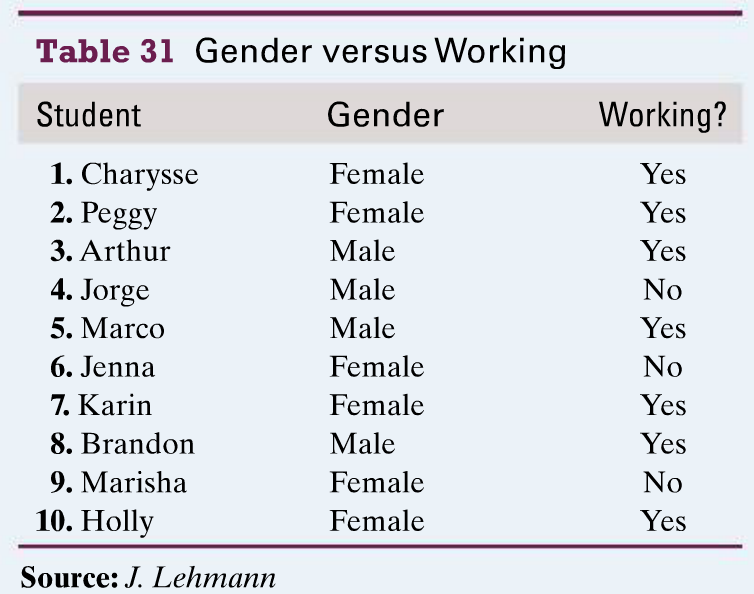
\includegraphics[scale=0.5]{ReviewSec32}
\end{center}
Use it to answer the following questions:
\begin{enumerate}
	\item Create a two way table that represents gender vs working
	\item What proportion of students are Female \textbf{\underline{AND}} Work?
	\item What proportion of students are Female \textbf{\underline{OR}} work?
	\item Create a multibar graph.
	\item What proportion of Male students work?
	\item What proportion of students work?
	\item What proportion of students are male?
\end{enumerate}

\subsection*{Section 3.3}
The following data is the top 50 finishers of the women's New York City Marathon.
\begin{center}
	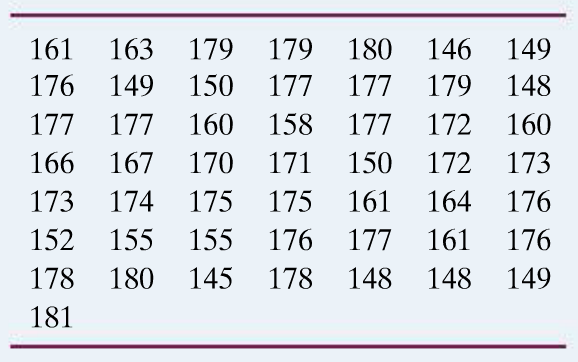
\includegraphics[scale=0.5]{ReviewSec33}
\end{center}
Use it to answer the following questions:
\begin{enumerate}
	\item Create a stem and leaf plot to represent the data.
	\item What is the frequency of the observation 148? In context of the problem, what does this mean?
	\item Which observation has the greatest frequency?
	\item What type of data is this?
	\item What is the 87th percentile? What does it represent in this situation?
	\item How many observations are below 160?
	\item What percentile is the value 164?
\end{enumerate}

\subsection*{Section 3.4}
The following data is the top 24 hits of smartphone prices on Amazon.
\begin{center}
	\includegraphics[scale=0.5]{ReviewSec34}
\end{center} 
Use it to answer the following questions:
\begin{enumerate}
	\item Create a histogram with a class width of 25 and a lower class bound of 25.
	\item Describe the shape of the distribution.
	\item Are there any outliers? If so, why is there an outlier?
	\item What proportion of smartphones have prices between \$95 and \$114?
	\item Calculate the mean, median, mode, range and standard deviation for this data set.
\end{enumerate}

\subsection*{Section 4.1}
\begin{figure}[h!]
\centering
\begin{subfigure}{.5\textwidth}
  \centering
  \includegraphics[scale=0.45]{RevSec411}
  \caption*{(d)}
\end{subfigure}%	
\begin{subfigure}{.5\textwidth}
  \centering
  \includegraphics[scale=0.45]{RevSec412}
\end{subfigure}
\end{figure}

\begin{figure}[h!]
\centering
\begin{subfigure}{.5\textwidth}
  \centering
  \includegraphics[scale=0.45]{RevSec413}
\end{subfigure}%	
\begin{subfigure}{.5\textwidth}
  \centering
  \includegraphics[scale=0.45]{RevSec414}
\end{subfigure}
\end{figure}

\noindent
Use the above to answer these questions.
\begin{enumerate}
	\item Describe the shape of each of the histograms
	\item How is the mean related to the median in each of the histograms?
	\item Which histograms would we use the mean and standard deviation to describe?
	\item Which histograms would we use the median and range to describe?
	\item Estimate the mean and median for each of these histograms.
\end{enumerate}

\subsection*{Section 4.2}
\begin{center}
	\includegraphics[scale=0.5]{RevSec42}
\end{center}
Use this to answer the following questions:
\begin{enumerate}
	\item Estimate the proportion of scores that are between 15 and 25 points.
	\item Estimate the proportion of scores that are between 10 and 30 points.
	\item Estimate the proportion of scores that are between 5 and 35 points.
	\item Estimate $s$.
	\item What rule did you use to estimate $s$? 
	\item What is another name for the things you calculated in Questions 1, 2 and 3?
\end{enumerate}

\subsection*{Section 4.2}
\begin{center}
	\includegraphics[scale=0.5]{RevSec421}
\end{center}

\begin{enumerate}
	\item Estimate $M$
	\item Estimate $\overline{x}$
	\item Estimate $s$
	\item Estimate $R$
	\item How did you find the answer to Question 3?
	\item Using your estimate to $s$ and $\overline{x}$ calculate 1, 2 and 3 standard deviations from the mean.
\end{enumerate}

\subsection*{Section 4.3}
Use the following boxplot to answer some questions.
\begin{center}
	\includegraphics[scale=0.5]{RevSec44}
\end{center}

\begin{enumerate}
	\item Describe the shape of the boxplot.
	\item Estimate the 25th percentile. In context of the problem, what does this mean?
	\item Estimate the percentile of a \$20 thousand dollar loan. What does this mean in context of the problem.
	\item What is the largest loan?
	\item What is the IQR?
	\item A student says that there are more loans for \$20-\$35 thousand dollars. What would you tell this student?
	\item How much data is between the loan amounts \$0 and \$8.3 thousand dollars? How do you know?
\end{enumerate}



\end{document}































